\chapter{On topic analysis for population displace signal extraction from news media}

\begin{abstract}
The world has witness mass forced population displacement across the globe. According to United Nations reports, the number of people displaced by conflict and persecution continues to soar reaching 65.3 million, with 12.4 million newly displaced in the recent years \cite{unrefugeeagency2016}. The population displacement requires accurate planning and resource allocation across the borders to mitigate the humanitarian crisis. The humanitarian planning involves following of population movements, resource allocation, and forecasts. The population movement is usually triggered by a set of event that pushes the individuals out of their place of living. The news media articles are considered to be an excellent source of world events. In this work, we analyze a large news media corpus to extract and evaluate the forced population displacement signals such as environmental, security, political, economic, and religious. These factors have pull/push effect on the population movement in the geographical regions. The application of topic modeling is an effective approach to extract the latent structure of the text corpus. The experimental studies show the optimized topic models with a high level of coherence can be extracted from the news corpus and can be further aligned with the population displacement factors.    
\end{abstract}

\section{Introduction}

In the recent decade, there has been an explosion in the amount of available digitized data about all sort of human activities. As the technologies evolve to handle more data, the amount of information grows exponentially. The information comes in different form and shape, pertaining various aspects of human life. One form of information about human activities comes in the form of news media, which is generated by the reporters and news agencies across the globe. The news media articles contain the information about the state of affairs as described by the news reporters. News agencies produce a vast amount of information about the events happening every day, covering from local to international affairs. The content of news articles ranges from social, political, economic events,  to reports on the environmental events. As a result, the news media articles collected from across the globe are a source for analyzing the world events. 

According to United Nations high commission for refugees, the number of population displacement has soared reaching 65.3 million \cite{unrefugeeagency2016}. An estimated  12.4 million people are displaced due to conflict or persecution in recent years. Population movements to this scale are usually triggered by a set of events that force the population out of their homes. The news media is a great source to extract the latest events in the region. One approach to analyzing large text corpus to uncover the latent thematic patterns is the application of topic modeling \cite{Blei2003}. The latent themes in the news media can help us to understand the population displacement triggers and signals, which are reflected in the news media reports. 

In this study, we take the challenge of extracting and analyzing the population displacement factors appearing in the new media. The focus of this study is the population movements originating in the Middle East, specially in Iraq and Syria. We gather the large news media article corpus spanning from 2012 to 2017 and apply various topic modeling methods to extract the most coherent set of topics. We also expand on the two-layer dynamic topic modeling approach which uses Non-negative Matrix Factorization (NMF) \cite{Lee1999} and evaluates the results with other methods such as Latent Dirichlet Allocation LDA and Latent Semantic Analysis LSA. 

The objective of this study is to answer the following research questions:


\begin{itemize}
\item Can a large corpus of news media articles reveal the forced displacement factors and signals
\item Evaluate topic modeling techniques to extract the representative forced displacement factors
\item Analyze and evaluate the correlation of events extracted from topic modeling to the real world events
\end{itemize}


\subsection{Detecting Event Magnitude}
In a recent work, \cite{Agrawal2016DetectingTM} introduced an effective model to detect events in large  news corpus. The objective of the approach is to analyze the magnitude of a given event from the text documents. The proposed model is designed to efficiently track the magnitude of the target event, which is defined previously. An event may be defined as 'violence', 'disease' or 'politics', which are defined by the collection of seed words. These seed words are designed to capture the context of related words to the general topic of the event. The goal of model is to evaluate the document and output the magnitude of the event based on the similarity of the document context and the seed words defining the event. The magnitude of the event is defined by the assigning an \textit{EventScore} to the document based on the measured similarity of the document and the seed words.  

To assign magnitude value to the event in the  document, \cite{Agrawal2016DetectingTM} first obtain the average word similarity between $w_i$ and \textit{E}, where \textit{E} is a set of seed words pertaining an event. 

\begin{equation}\label{eq:simEQ}
Sim (w_i, E) =  \frac{1}{\mid Y\mid}    \sum_{j=1}^{m} Sim(w_i, y_j)
\end{equation}

The $Sim (w_i, y_j)$ in equation \ref{eq:simEQ} can be calculated with three different methods: 1- Normalized Pointwise Mutual Information (NPMI), 2- Continuous Bag-of-Words (CBOW) and 3- Skip-gram (SG). Using the Word2Vec embedding \cite{Mikolov} trained on the text corpus provide the missing context to calculate the \textit{EventScore} based on the similarity $Sim (w_i, E)$ in the previous step (Equation \ref{eq:EventScore}). 

\begin{equation}\label{eq:EventScore}
EventScore (d_k, E) =  \frac{1}{\mid n\mid}    \sum_{i=1}^{n} Sim(w_i, E)
\end{equation}
\vspace{-1em}
\begin{equation}\label{eq:EventScore1}
EventScore (t_s, E) =  \frac{1}{\mid D\mid}    \sum EventScore(d_k, E)
\end{equation}

The event score of an article $d_k$ with $n$ token is computed for specific window of time. To arrive at the event score for a specific window of time $t_s$, $EventScore(d_k, E)$ for all documents in $t_s$. The model is validated by manually assigning an event magnitude score to set of training documents, and evaluate the expert labels correlation with the $EventScore (d_k, E)$ through Pearson's correlation measure. The preliminary evaluations on limited set of news article from the Expandable Open-Source (EOS) collection shows strong correlation between the expert and $EventScore.$ However, the work is limited by the choosing of seed words to define the target event and is not sensitive to range of topics in the news media documents. The approach is based on the assumption that the target events can be observed in the corpus, with limited set of defining seed words. In this works, we take a different view on the event, and define the events on broader level in the topic space. More on this in next section. 

\subsection{Exploring the Political Agenda through Dynamic Topic Modeling}
To analyze the evolution of topics over time, \citet{Greene2016} demonstrate the application of dynamic topic modeling. Topic modeling have been adopted in the political science applications to analyze political related documents. The political and social science setting requires analyzing wide range of documents, which are dynamic and changing over periods of times. Leveraging the latent themes and topics can help the politicians and social scientists uncover the hidden signals on the large corpus of data. The dynamic topic modeling introduced in \cite{Greene2016} is based on two layers Non-negative Matrix Factorization (NMF). NMF is an unsupervised learning method which reduces the dimensionality of non-negative matrices. The clusters forming from NMF calculation are interpreted as topics in the text corpus. 

The goal of dynamic topic modeling is to analyze the temporal data. The topics and the content of the documents change over time, and the goal is to identify the topics across the whole corpus, as well as the short-lived topics that appear only in a portion of the corpus. 

The dynamic topic model introduced in \cite{Greene2016} has two layers. In layer 1,  NMF is applied on the \textit{time windows} of the text corpus, which is a set of documents in from fix duration of time (i.e. monthly, quarterly).  Layer 1 produces a set of successive window topic models. In the Layer 2, a new condensed representation of the original corpus is generated to analyze the evolution of topics. The dynamic topics models produced from Layer 2 is evaluated by topics coherence score, which refers to the level of semantic similarity between the top terms in the topic. Furthermore, topics are analyzed and evaluated on case study basis in the domain of political debates in European parliament. 





\subsection{Topic Modeling}
Topic modeling is an effective method to process large amount documents. The method allows for discovery of a distinct set of topics among the corpus. A topic modeling approach can connect the words with similar meaning and form topics. 

% The objective of topic modeling is to extract

In this section, we describe some the popular topic modeling methods including Latent Semantic Analysis (LSA),  Hierarchical Dirichlet Process (HDP), and Latent Dirichlet Allocation (LDA). 



\begin{figure}[t]
\caption{Topic Modeling - Documents are represented as a mixture of a pre-defined number of topics (K), and topics are represented as mixture of individual tokens in dictionary}
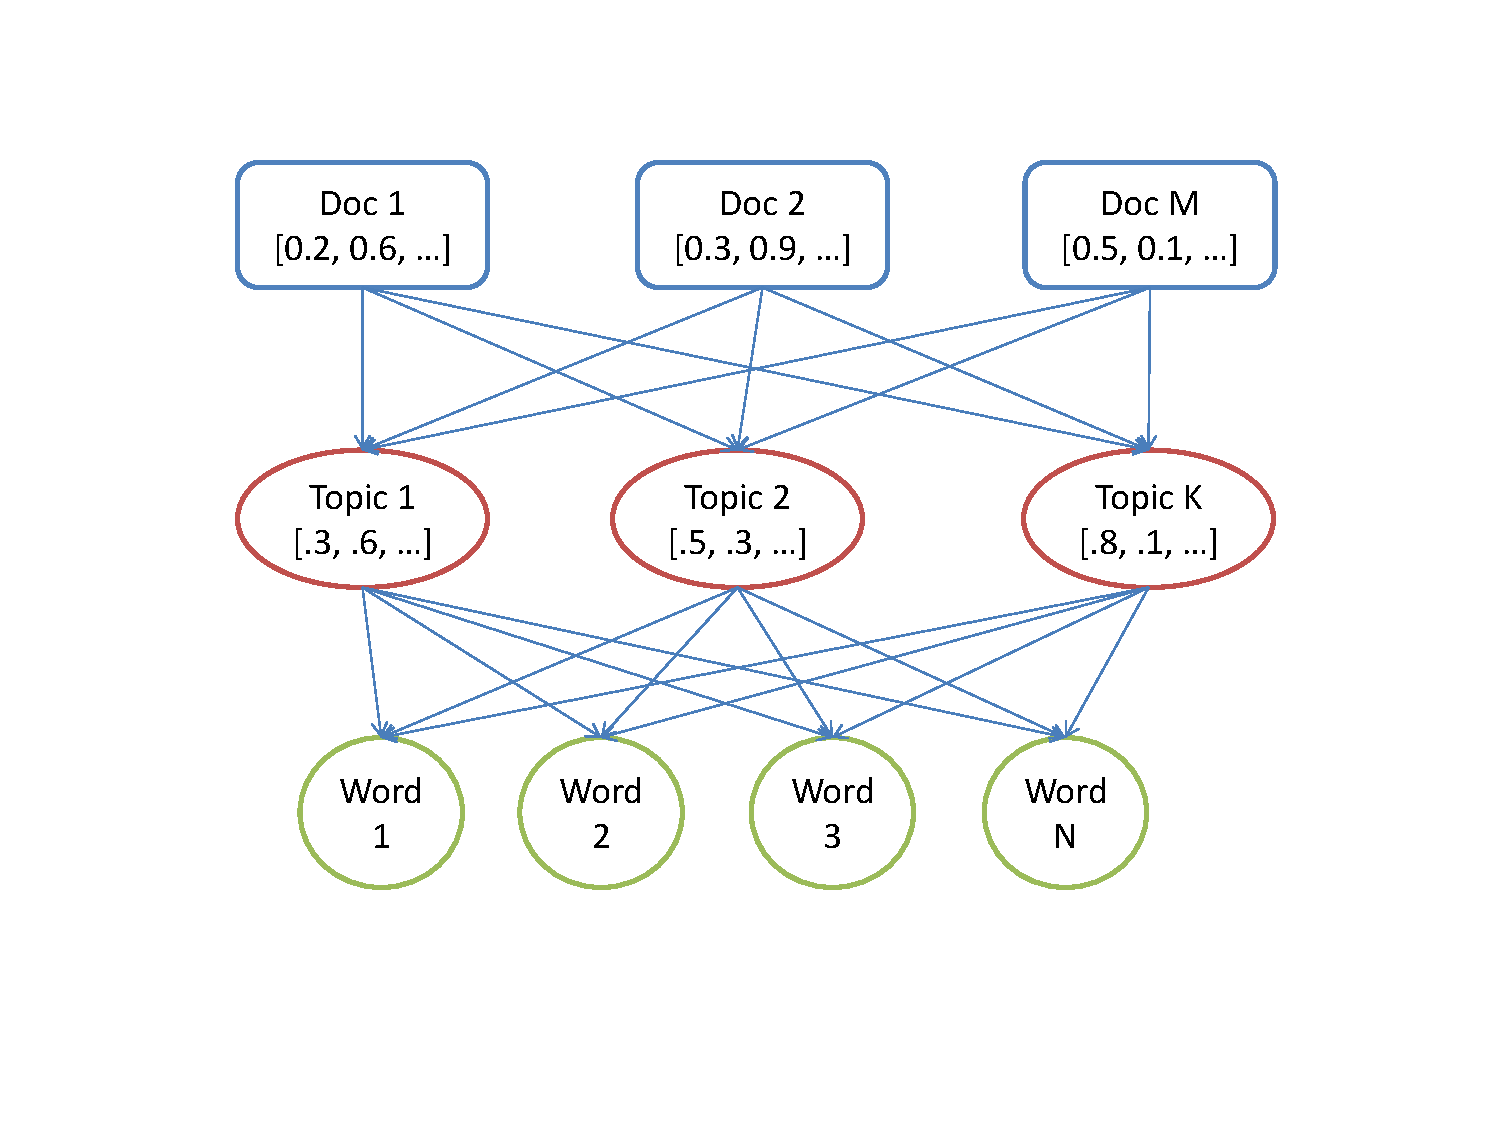
\includegraphics[scale=.5]{img/topicmodeling.pdf}
\centering
\label{fig:topicmodel}
\end{figure}

\subsection{LSA (Latent Semantic Analysis)}
The LSA is a text analysis algorithm that builds a semantic space from a text corpus.  This semantic space is then used to compute the similarity between the documents in the corpus. The objective is to create a vector-based representation of the text. At its core, LSA uses Singular Value Decomposition (SVD) to create the latent space representation \cite{Deerwester}. The probabilistic topic models have also proven to be effective, which led to the introduction of Probabilistic Semantic Analysis (PLSA) \cite{Hofmann2001}. In the probabilistic semantic space, a topic is a probability distribution over the words and documents being represented as mixtures of topics. This property of probabilistic allows a topic model to behave as a generative model for documents \cite{Ocallaghan}. 


\subsection{Hierarchical Dirichlet Process (HDP)}
Earlier works have shown that the hierarchical Dirichlet process(HDP) is an effective mixed membership model for unsupervised analysis of the grouped data\cite{WhyeTeh2006}. The HDP provides a non-parametric topics model with based on the view that documents are observed words, mixture components (i.e. topics) distribution over terms of the document. Similar to the overall objective of other topics models, HDP topic model finds a low-dimensional latent structure that is suitable for tasks like classification and topic analysis. The main difference of HDP from other topic model counterparts is that it infers the number of topics from the data. The online variational Bayes for HDP \cite{pmlr-v15-wang11a} is a popular method to optimize the variational objective function wit stochastic optimization. This enables online HDP to provide the speed of online variational Bays with the modeling flexibility and scalability of the HDP.


\subsection{LDA (Latent Dirichlet Allocation)}
LDA belongs to the group of generative probabilistic models for documents. Based on an intuitive idea that each document is comprised of a mixture of topics, and each topic is a discrete probability distribution of how likely each word is to appear on a given topic (Figure \ref{fig:topicmodel}). Given set of documents $W = \{w_1, w_2, ...,  w_d\}$, to generate a word token $w_n$  from document d, a discrete topic assignment $z_n$ is drawn from a document-specific distribution over the T topics $\theta_d$. This value is drawn from a Dirichlet prior with hyper parameter $\alpha$. The inference task in topic models is generally defined as inferring the document proportions $\{\theta_1, ... \theta_D\}$ and the topic-specific distributions $\{\phi_1, ... ,  \phi_T\}$ \cite{Mimno}. Figure \ref{fig:ldamodel} shows the plate notation for the graphical LDA topic model.


\begin{figure}[t]
\caption{Plate notation of LDA }
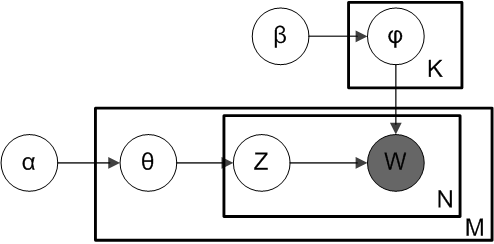
\includegraphics[scale=.5]{img/lda.png}
\centering
\label{fig:ldamodel}
\end{figure}

\subsection{Machine Learning for Language Toolkit - MALLET}
Building on foundations of LDA, \cite{Griffiths} proposed using a Dirichlet prior on topic-word distribution $\phi$, with additional hyper parameter $\beta$. Further, \cite{Griffiths} used collapsed Gibbs sampling to estimate the topic space distribution indirectly. This method iteratively estimates the probability assignment of each word to the topics, conditioned on the current topic assignment of all other words. The popular topic modeling toolkit MALLET \footnote{Mallet toolkit \url{http://mallet.cs.umass.edu/}} is based on LDA with Gibbs sampling.


\subsection{Non-Negative Matrix Factorization (NMF)} \label{NMF}
Non-negative matrix factorization (NMF) \cite{Lee1999} is a widely used approach for the analysis of high-dimensional data. The objective of NMF is to extract meaningful features from a set of non-negative sparse vectors. The NMF is successfully applied to different applications, such as image processing, hyper-spectral imaging,  and text mining.  Here we focus on the property of NMF to identify topics in a given set of documents and classify the documents among the underlying topics.

Let each column of the non-negative data matrix $X \in \mathbb{R}$ represents a document and each row to a word in the dictionary. In this matrix, the $(i, j)^{th}$ entry corresponds to a number of times the $i^{th}$ word appears in the $j^{th}$ document. Each column of the matrix X is the word count of a $j^{th}$ document. In practice, the bag-of-word is replaced by term frequency - inverse document frequency (TF-IDF) representation of the document. The use of TF-IDF pre-processing has shown to help results of NMF by down-weighting the contribution of high-frequency terms while boosting the effect of rarer terms in the corpus \cite{Greene2016, Gillis2014}. The matrix X is rather sparse since most of the documents only have a small subset of the dictionary terms.

Given matrix X and factorization rank $r$, NMF decomposition generates two non-negative factors W and H, where $X \approx W H$ (Eq. \ref{eq:nfm}) \cite{Lee1999}. 

\begin{multline}\label{eq:nfm}
\underbrace{X(:,j)}_\text{jth document.} \approx \sum_{k=1}^{r} \underbrace{W(:,k)}_\text{kth topic.} \underbrace{H(k,j)}_\text{ weight of $k^{th}$ topic in $j^{th}$ document.} , 
with W \geq 0 and H \geq 0.
\end{multline}

The results NMF decomposition can be interpreted by examining the W and H matrix. Because W is non-negative, each column of W can also be interpreted as a bag-of-words representation of the document.

\begin{figure}[ht]
\centering

\includegraphics[scale=.7]{img/NMF}
\label{fig:NMF}
\caption{NMF factorization}
\end{figure}

 At the same time, since weights in linear combinations are also non-negative, $H \geq 0$, the union with sets of words in W can approximate the original document. Since the number of documents (columns in X) is much larger than a number of basis elements (columns in W), the elements of W contains the set of words found simultaneously appearing in multiple documents. The weights in linear combinations, matrix H, assign the documents to different topics. Therefore, NMF  can identify the topics across the documents and classify each document according to the topics it belongs to. Inspired by the work done in \cite{Greene2016} to extract dynamic topics, we apply NMF on time-windows of news media corpus to extract the evolving topics. 
 
 
\section{Methodology}

\subsection{Topic Coherence Analysis}
Quantifying the coherence of the topics extracted from topic modeling methods is a crucial part of this research. The primary concern about the efficiency of the statistical topic modeling is the is the presence of poor and obscure topics in the results.  Topics with mix and loosely related concepts usually fail to generate meaningful insight for the users. As  \cite{Mimno} observed, there is a strong relationship between the size of topics and quality of the topics judged by domain experts. This is because as the number of topic increases, the quality of word distribution constituting the topic decreases. At the same time, the lower number of topics may result in an undesirable generalization of topic distribution in the corpus.  

Recent works on the evaluation of statistical topic models have focused on topic's semantic coherence \cite{Mimno, Ocallaghan, Roder2015}. In this work, we use the topic coherence measure introduced by \cite{Ocallaghan, Roder2015}.

\textbf{TC-W2V} is a distributional semantics measure introduced by \cite{Ocallaghan}. TC-W2V measure is based on the popular word2vec \cite{Mikolov} word embedding technique.  The words vectors are generated using the word2vec Skip-gram model using the corpus.  The same set of pre-processing is applied on the corpus used to train word2vec model as used in generating topic models. In this method, the coherence score is the mean pairwise Cosine similarity of two term vectors generated by Skip-gram model (Eq. \ref{eq:tc_w2v}). 

The topic descriptor is generated based on the number of $N$, a where set of highest-ranking terms from the topic's basis vector in $W^k$ is calculated to describe the topic. 


\begin{equation}\label{eq:tc_w2v}
TC-W2V = \frac{1}{(_{2}^{N})}  \sum_{j=2}^{N} \sum_{i=1}^{j-1} similarity (wv_j, wv_i))
\end{equation}

Another recent work on topic coherence measure is the unifying framework proposed by \cite{Roder2015}. The framework represents the coherence measures as a composition of parts, where the objective is to achieve higher correlation with human judgments. The composition parts can be freely combined, which enables exploring variety of existing similarity measures techniques. The framework has four segments at its core: segmentation of words subsets, probability estimation, confirmation measure, and aggregation (Figure \ref{fig:coherence}). The stages of unified framework are briefly described below. 
\begin{itemize}
    \item Segmentation of word subsets. The coherence of a word set is the  degree that a subset is supported by another subset. Based on this, the result of segmentation of a word set $W$ is a set of pairs of $W$ subsets to produce $S$.  

    \item Probability estimation pertains to the method to derive the probabilities from the corpus. Different methods are available to estimate the probabilities. \textit{Boolean document} $\rho_{bd}$ estimates the probability of single word as a number of documents in which the term is observed. Other methods, such as \textit{Boolean paragraph} $\rho_{bp}$ and \textit{Boolean sentence} $\rho_{bs}$ are similar to the $\rho_{db}$ except that document paragraphs and sentences are used for the measurement. \textit{Boolean sliding window} $\rho_{sw}$ determines the word counts based on the defined sliding window increments. In each sliding window, a virtual document is created and \textit{Boolean document} is applied to calculate the word probabilities. 
    
    \item Confirmation measure takes the output from word subsets $S$ and computed probabilities $P$ to calculate the agreements $\varphi$ of pairs of $S$. The confirmation measure can be done directly \cite{douven2007} or indirectly as proposed in \cite{Aletras}. 
    
    \item Aggregation stage is the process aggregating the all confirmations of all subset pairs to generate a single coherence score.
    
\end{itemize}

\begin{figure}[t]
\caption{Unifying coherence framework \cite{Roder2015}.}
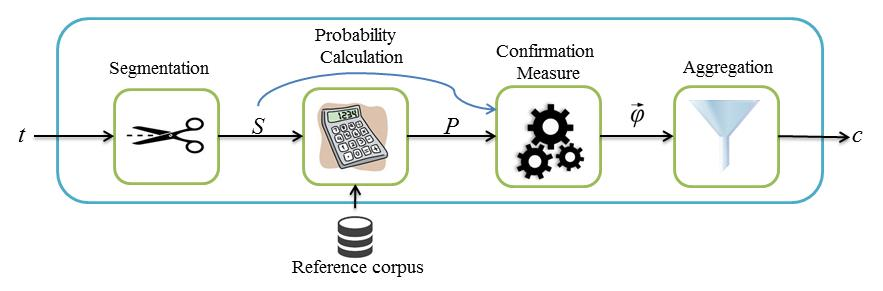
\includegraphics[scale=.5]{img/coherence.jpg}
\centering
\label{fig:coherence}
\end{figure}


\subsection{Topic model generation}
In order to broaden the extent of topic analysis and establish a baseline on news media corpus, we generate and evaluate some of the classical topic modeling methods. Here we describe the generation, and evaluation process of following topic modeling methods: LDA, LSA, and LDA Mallet (Gibbs sampling). 
First, we describe the process of generating the LDA models based on the optimal topic number. To identify the optimal topic number $k$,  we first generate LDA models with a number of topics in the range of $k \in \{10, 30\}$ with an increment of two. The entire corpus is used to generates and store a range of  LDA model as defined by the range of $k$.

To find the optimal $k$ in the topic number range, we apply topic coherence measures to choose the best result. Here, we apply two different topic coherence measure described in section 4.2. The similar steps are taken to generate the LSA and LDA model using Gibbs sampling. We used the same range of topic number $k$ to generate and evaluated models across all methods (LDA, LSA, and LDA using Gibbs sampling). 
At this stage, we analyze the application of classical topic models on the entire corpus and the dynamic time windows. This baseline examines the ability of widely used topic modeling methods to deal with large news media corpus and provides an initial assessment of the topic space.

\textbf{Baseline} In this study, we take the LDA Mallet as the strong baseline for evaluating the performance of our models. LDA and and it's Gibbs sampling variation available in Mallet toolkit has been reported to be among the high performing probabilistic topic models \cite{Griffiths, Greene2016}.  

\subsection{Dynamic topic learning}
In this section, we describe the dynamic topic modeling introduced in \cite{Greene2016}. The dynamic topic model involves two layers matrix factorization. Layer 1 involves getting the topic models from the time windows. The Layer 2 extracts the dynamic topic model across all time windows. \\
\textbf{Layer1}\\
The first step required in Layer 1 is to partition the data into a set of disjoint windows, $T \in \{T_1,  ...,  T_T\}$. The process described in section 5.3 produces 12 monthly time window collection for the year 2016-2017. The windows are demarcated by the beginning and the end of each month. Given the time window $T$, in the first layer, we apply NMF to a range of topic number $k$. The topic ranking $k_best$ in the range is selected by measuring the TC-W2V coherence score. The topic model $M_{K_{best}}$ is generated for each time window. The result of this process is a set of topic models $M \in \{M_1, ...,  M_T\}$ for each time window. The topic model set $M$ captures the topics exclusive to the short period of window size. Topic models at this layer can be views by the top word distribution representing the topic. \\
\textbf{Layer2} \\
The layer 2 requires the set of time window topic models $M \in \{M_1, ...,  M_T\}$ generate in layer 1. Given a topic model, a condensed representation of the original corpus can be constructed by viewing the rows of each factors $H_i$ from windows topic models. This is referred to as "topic documents". Each topic document contains non-negative weights indicating topic ranking "descriptive terms" for the window topic. The topic models describing a similar topic will have similar descriptive terms. The used of only top-ranking terms allows the dynamic layer to implicitly incorporate features selected in Layer 1.  The matrix B has a size of $n^{'} x m^{'}$ where $n^{'}$ is the total size number of "topic documents" and $m^{'}$ is a subset of an original number of terms (i.e. descriptive terms). 

After constructing matrix $B$, the second layer of NMF topic modeling is applied on this matrix to derive the dynamic models. Again, the topic number $k$ is selected by measuring the TC-W2V coherence score.  The result of second order matrix factorization can be interpreted as the top-ranked terms and the indication of the extend each window topic relates to the dynamic topic. 

\section{Experiment}

\subsection{Expanded Open Source (EOS) - News Media Collection}
The news media collection we used in this paper is collected by the GeorgeTown University researchers. The Expanded Open Source (EOS) collection is a vast unstructured archive of well over 700 million media articles gathered over years. The EOS collection is actively expanding by approximately 300,000 documents per day. The collection is expanded by searching over 20,000 Internet-based source (i.e. news outlets, official agencies, blogs) and covers over 46 different languages.

The EOS data is in XML format, and it is stored as one document per XML file. The XML file includes the following key elements: "Id", "SourceName", "PublicationDateTime", "Tile", "URL", "Language" and "text", which holds the main content of the document. For this research, we use only a portion of the EOS data selected from the news outlets. The data set is consist of 466,511 news articles with various topics spanning over late 2014 to mid 2015. This is a sample representative of the entire EOS, which is only sliced based on the published date. Figure \ref{fig:corpus_histogram} describes the document length characteristics of the data used for this experiment.

\begin{figure}[t]
\caption{EOS data set statistics.}
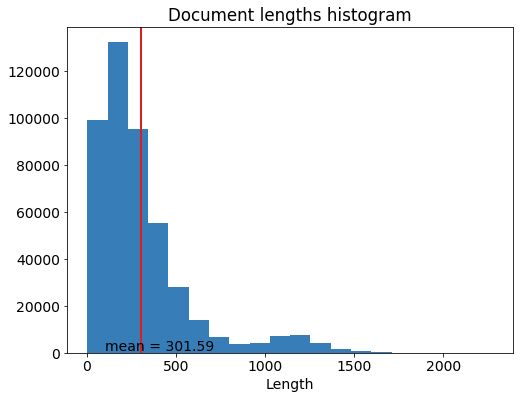
\includegraphics[scale=.6]{img/corpus_histogram.png}
\centering
\label{fig:corpus_histogram}
\end{figure}

\subsection{Data pre-processing}
In order to be able to scale to high volume corpus and apply a common set of pre-processing steps, we use pipeline framework to process the documents. The data pipeline frameworks refer to the multiprocess enabled data extraction and manipulation. More explicitly, our data pipeline includes the following: extraction, cleaning, pre-processing, and integration. 

In this work, we used the SpaCy \footnote{SpaCy \url{https://spacy.io/}} natural language processing library for Python. The objective of SpaCy framework is to provide the many common NLP functionalities supported by the underlying framework to handle a large load of data. In following, we provide a description of data pre-processing pipeline. The advantage of creating the data processing pipeline is two-fold: first, we can ensure that same set of pre-processing steps can be applied in generating the tokens for entire corpus, as well as generating time windows for dynamic topic modeling. Another advantage is to be able to process the large corpus in parallel, which significantly improves the pre-processing step.

The first step of pre-processing starts with the extraction of the data. The EOS data resides in XML format, which is parsed to get the document ID, publication date, and body. The output of extraction step is a document per line file format. In next step, we build the unigram representation of the text. The first step is to normalize the text by lowercasing all tokens. Second, we apply lemmatization on all tokens to get the roots of the token. In this scenario, we avoided doing any stemming as it often results in the generation of uninterpretable tokens that hinders topic coherence analysis by the end users. The normalized text output is used to build the bigram model of the corpus.

The bigram model will determine most likely concurrence of the tokens and generate bigram tokens. It is important to first generate the bigram model by observing the entire corpus and then process each document separately. This means that removing the unwanted tokens, such as stop words, is deferred to the latest stages of the processing pipeline. The next step in the pipeline if go through the corpus and store the bigram tokens for future use.  In this last stage, we remove the stop words from the final bigram tokens. The stop word list is consist of a set of English and Turkish stop words. This is because the EOS corpus has news articles from international media outlets. Further, we used a set of custom token exclude list to remove the unwanted tokens customer to the formatting of documents.

\subsection{Time window collection}
In order to be able to analyze the time evolution of topics in a large document collection, we first need to separate the documents into time-stamped bins. The achieve this, following by the previous works \cite{Sulo2010}, we divide the EOS data into a set of sequential non-overlapping time windows $\{T_1, ... , T_i\}$. Each time window bin is consist of sequentially ordered documents based on the published date information. Each bin has a set of non-overlapping documents divided on a monthly basis. 

\begin{figure}[t]
\caption{Time window stats}
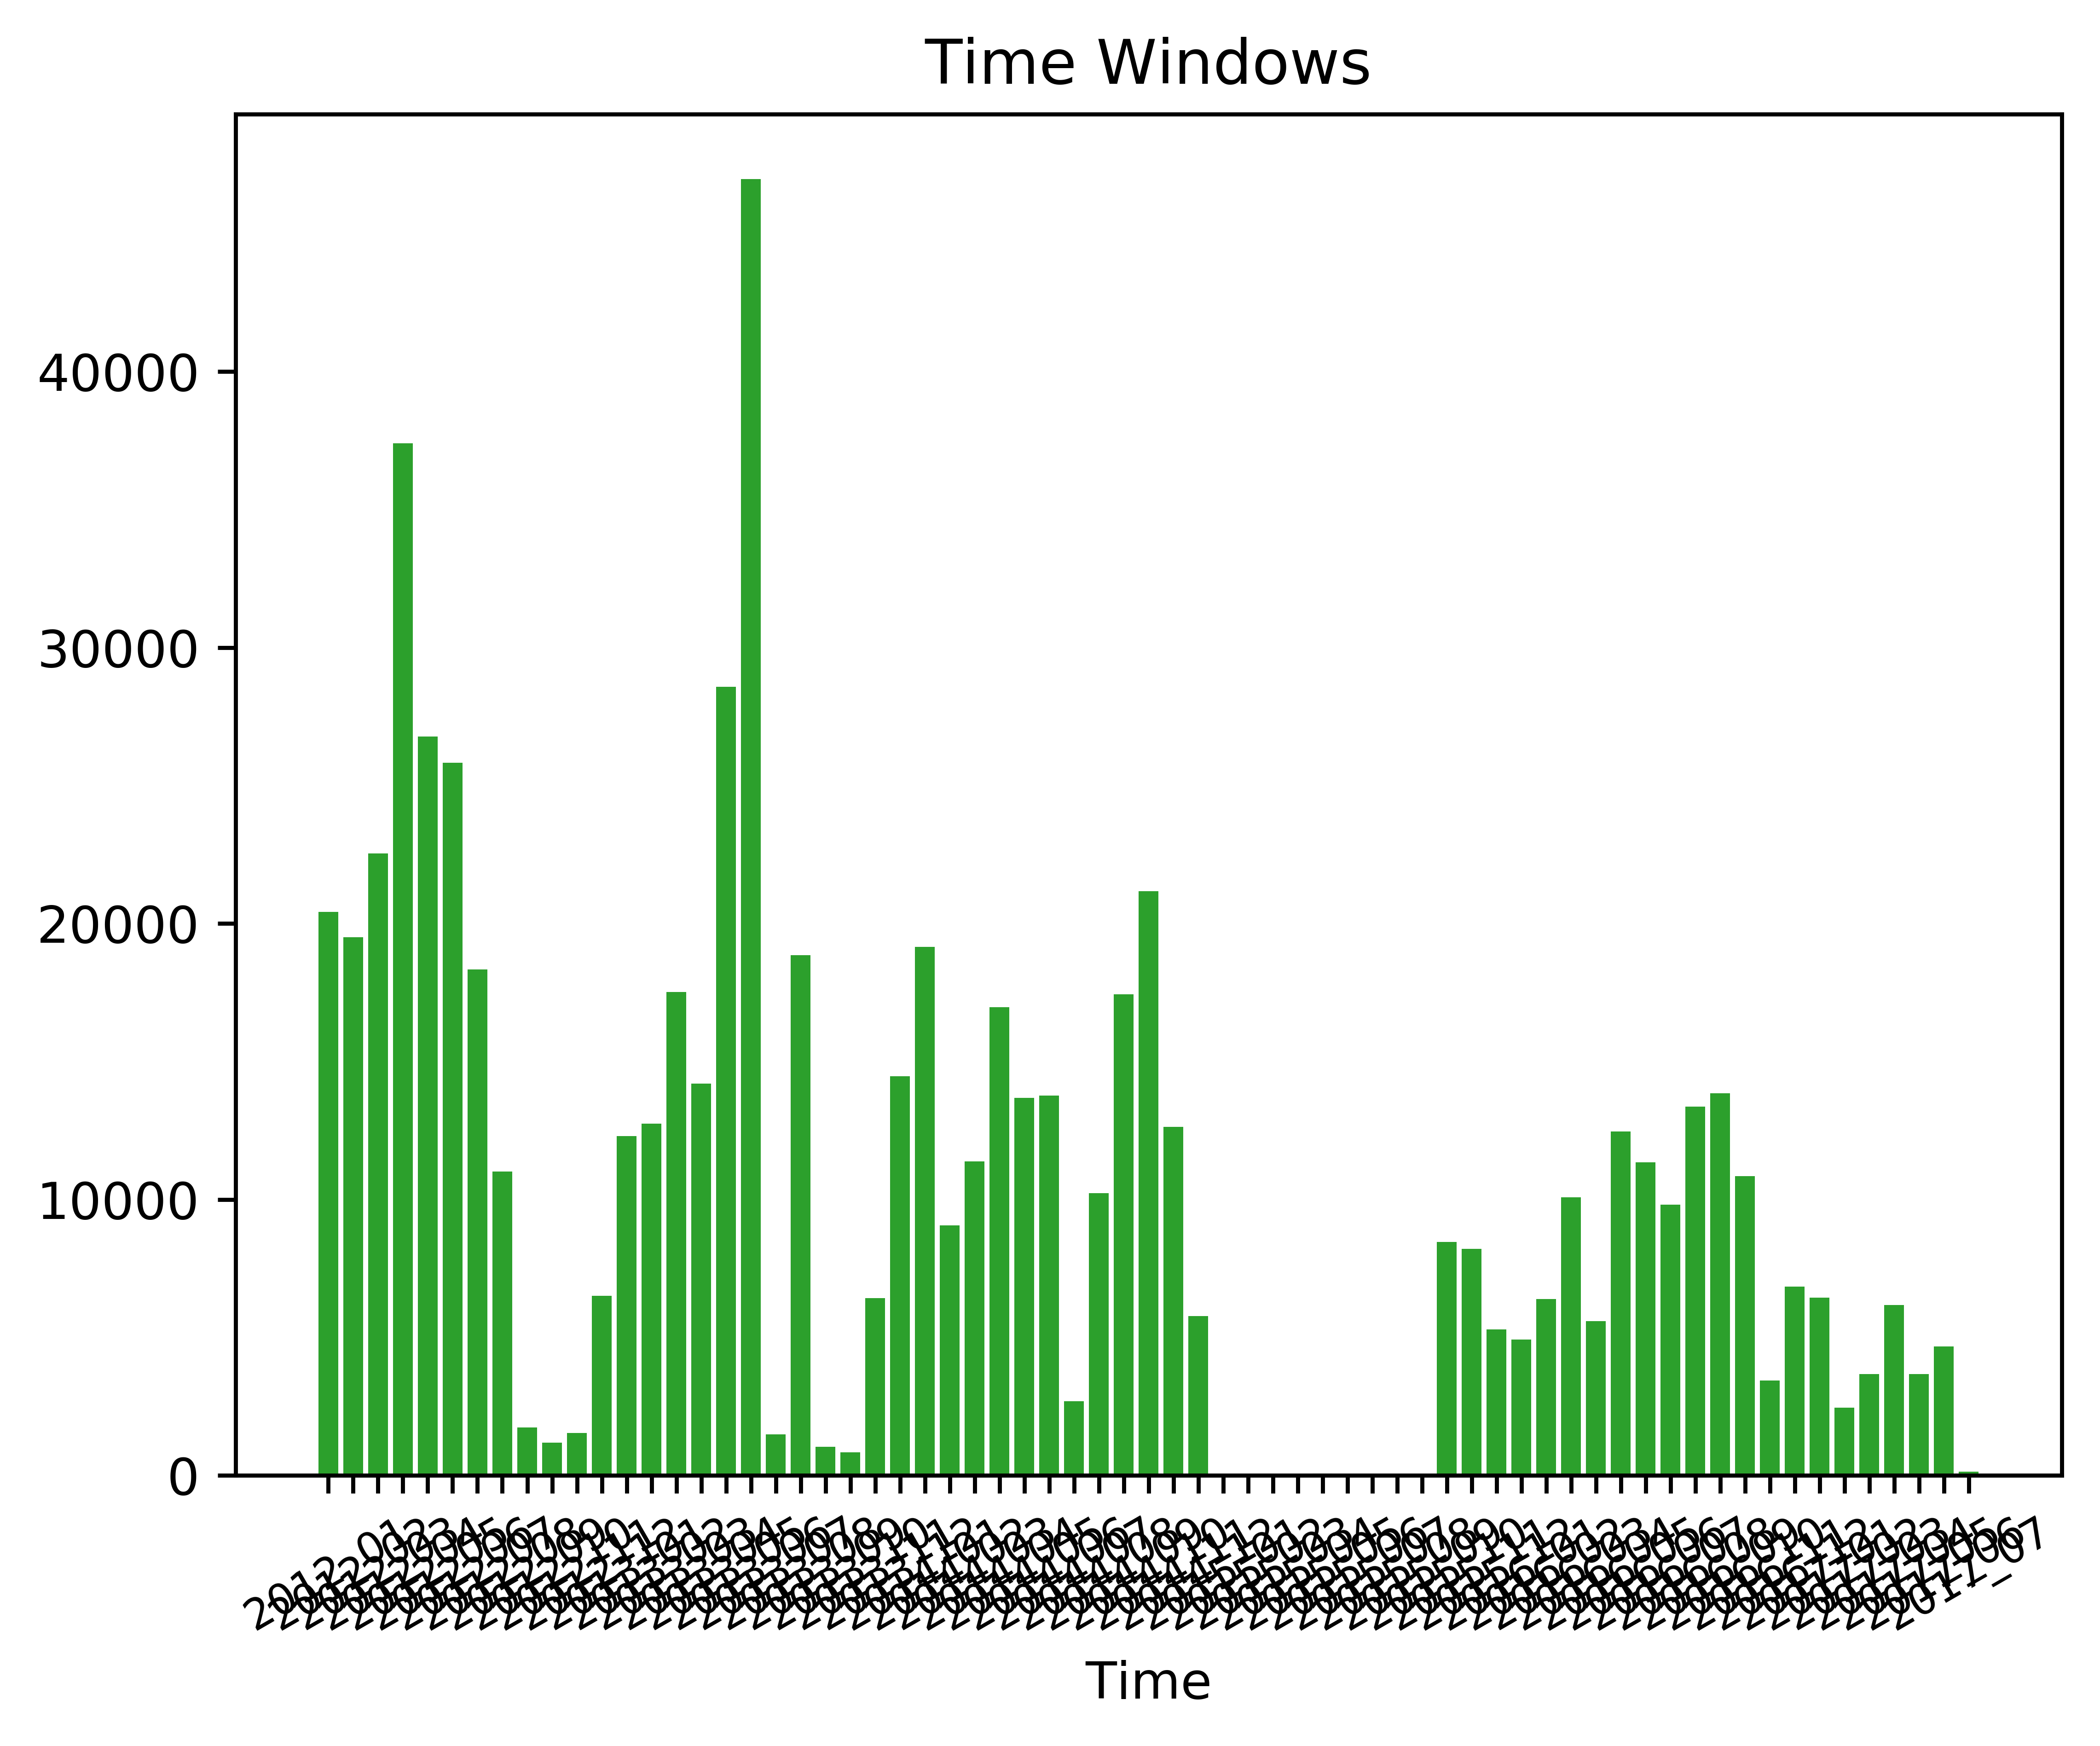
\includegraphics[scale=.8]{img/windows_corpus_info_2016_2017.png}
\centering
\label{fig:corpus_windows}
\end{figure}

The monthly time window bins ensure enough number documents are in each bin. The reason for creating a time window bins is two-fold: first, we are interested in the topical events in shorter window sizes. Second, The short-lived topics may be obscured by the generalized topics in the observed in entire collection. The monthly time window also allows us to identify more granular and short-term topics, as well as generalized topics over longer terms. Figure \ref{fig:corpus_windows} shows the distribution of number of documents in each time window. 



\section{Experimental Results}

\subsection{Windows Topic learning}
Here we describe the methods followed to generate and analyze the window topic models on EOS news media corpus. The window topics are the topics emerging from each separate time windows in the corpus. The windows topic analysis is useful in the analysis of the data to reveal the overall topics space of the corpus. The windows topics spaces tend to be sensitive to the local and short bursting topics in the large data since the models are trained on the subset of entire corpus. 

Training of the windows topic models starts with pre-processing the EOS corpus. The set of pre-processing steps described in section 5.2 is applied on the entire corpus, and then separated into time window bins as described in section 5.3. To analyze the window topic space, we use widely used methods: LSA, LDA and Mallet. We refer to the LDA method with Gibbs sampling as LDA Mallet since the best available implementation of the method is available through Mallet toolkit. LDA Mallet is one of the has reported to be strong baseline analyzing the performance of the topic models \cite{Greene2016}. 

First, we choose a range of topic number for LSA and LDA topic models. In this case, we choose $k$ to be a range between 10 to 30, with increments of two, that is $k \in \{10, 30\}$. Next, the LSA and LDA (both online and Gibbs sampling variations) models are generated using the window slice of the corpus. Training is done using multi-core processes to speed up the training. Using each topic modeling method, the model is generated given the range of topic numbers and stored.


% GRAPHS GO HERE
\begin{figure}[!ht]
  \centering
  \begin{minipage}[b]{0.45\textwidth}
    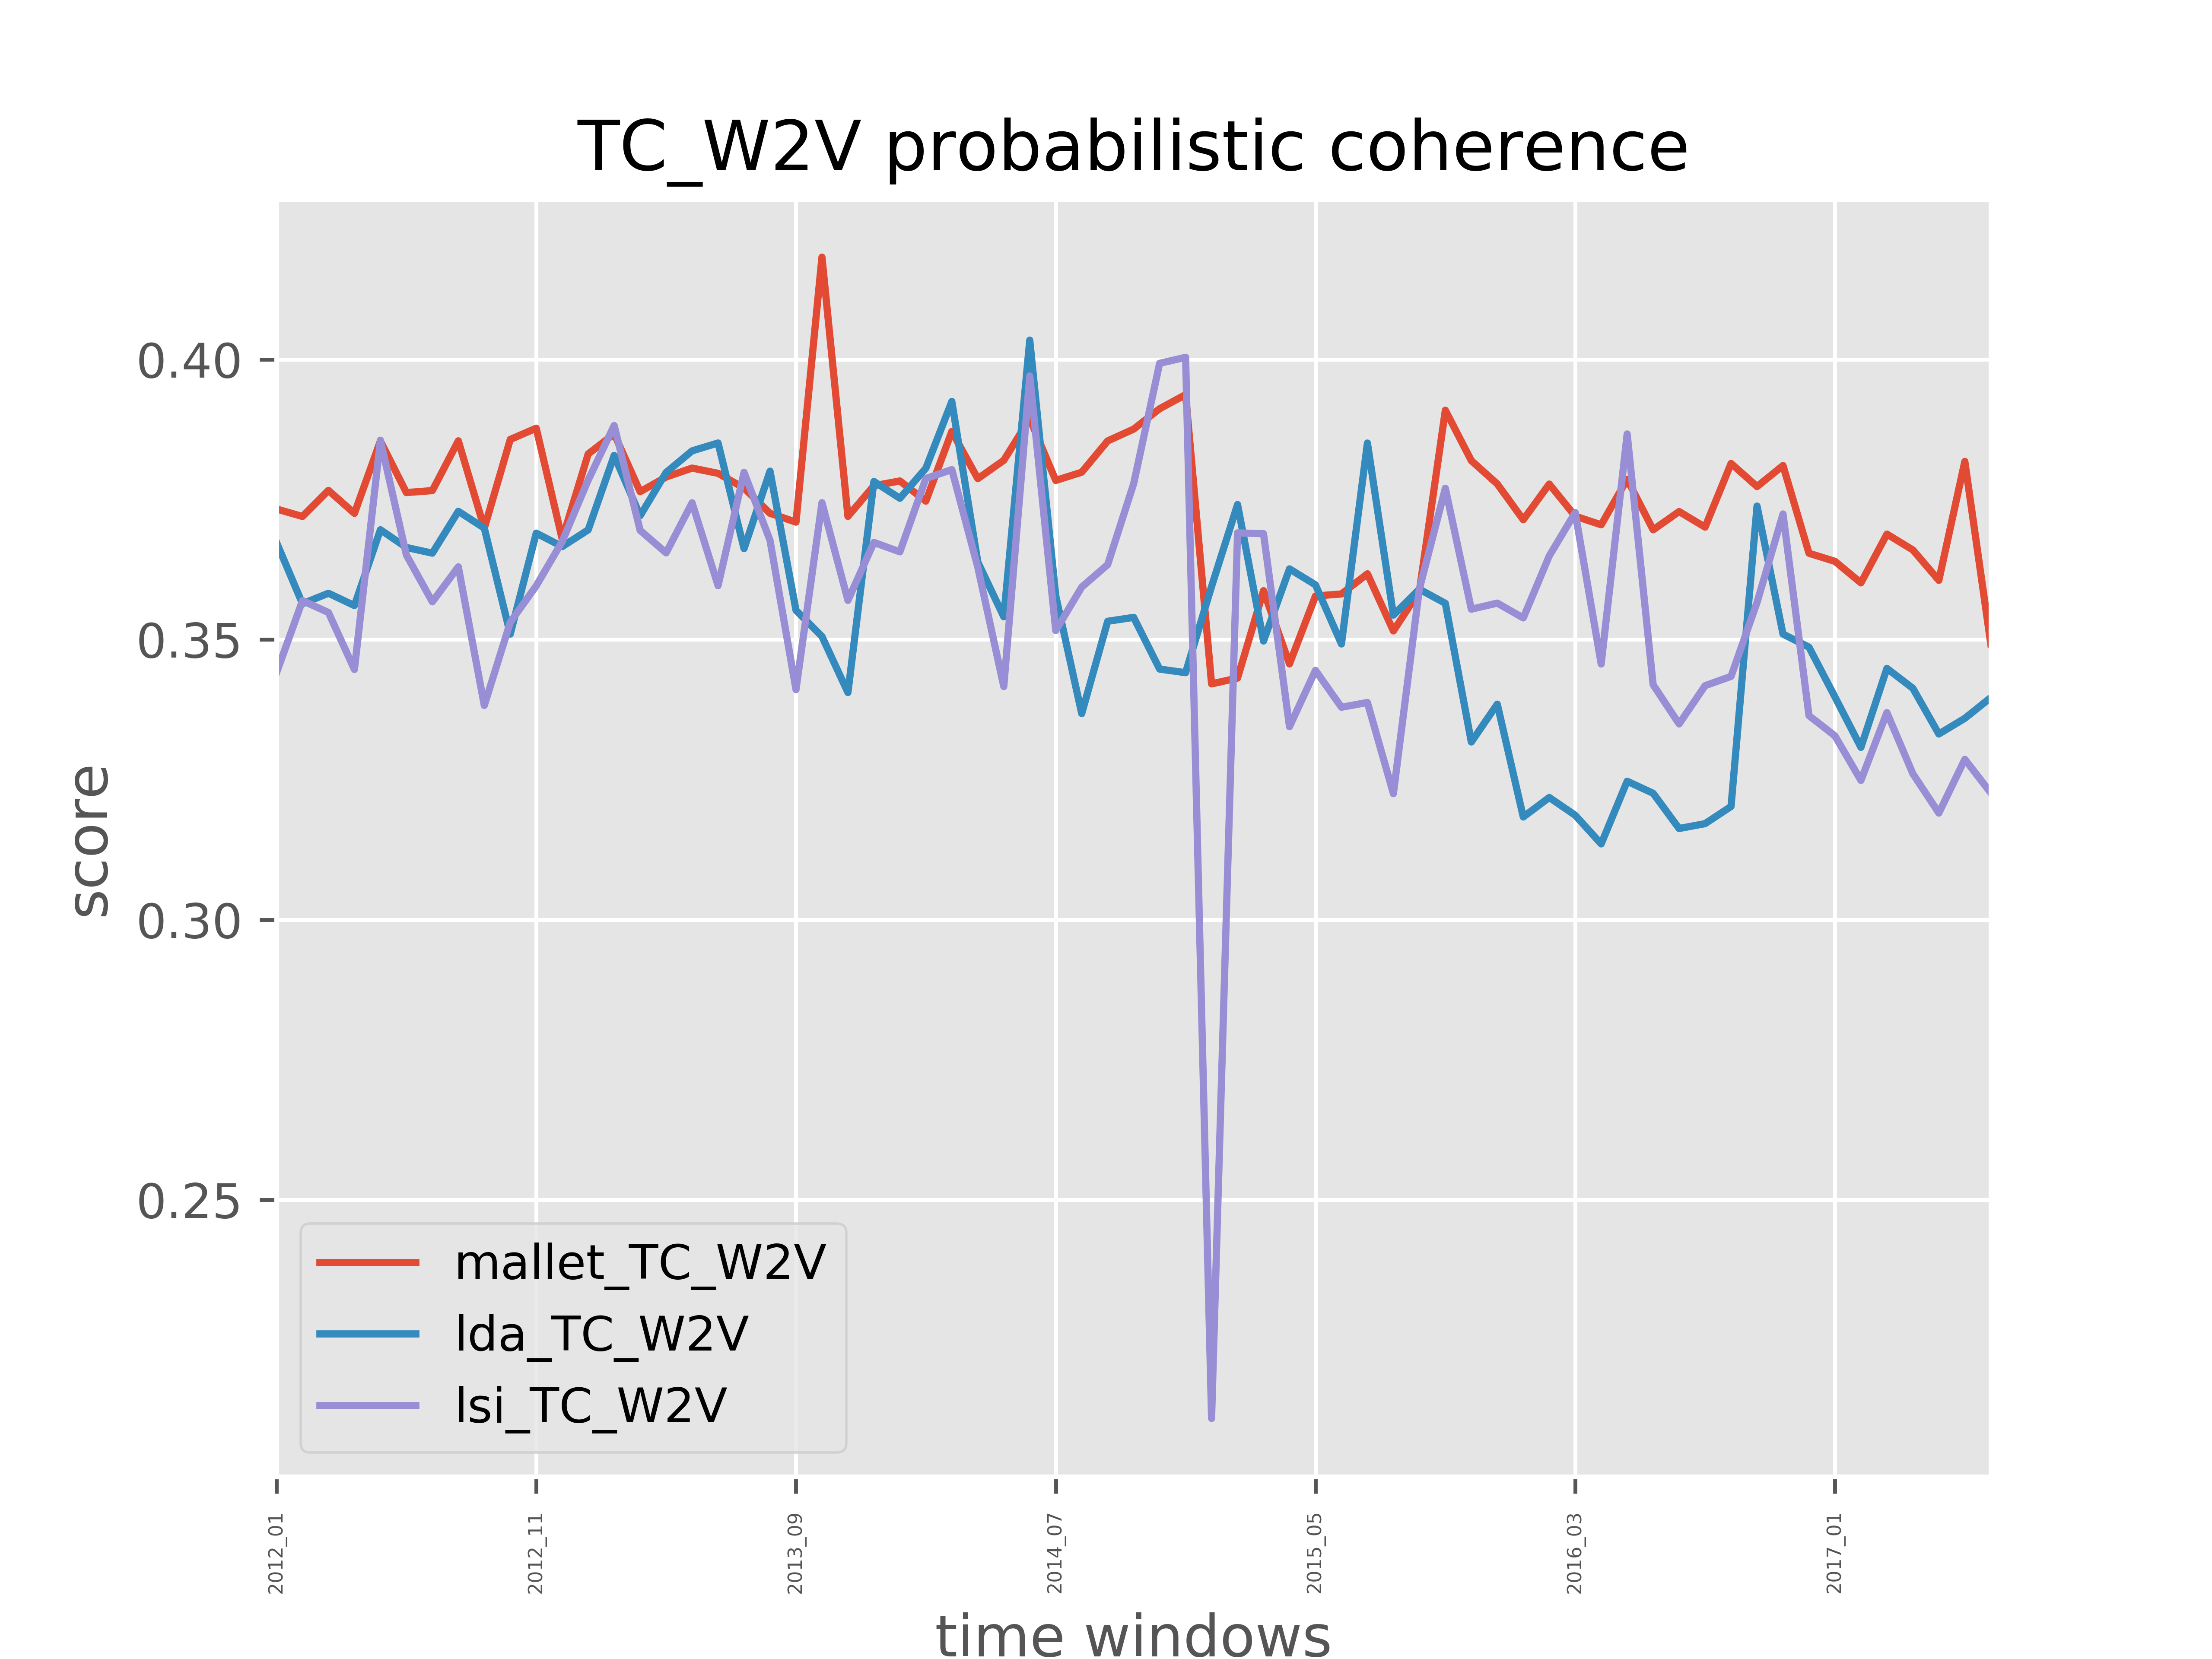
\includegraphics[width=\textwidth]{img/TC_W2V_probabilistic_all_coherence_plot.png}
  \end{minipage}
  \hfill
  \begin{minipage}[b]{0.45\textwidth}
    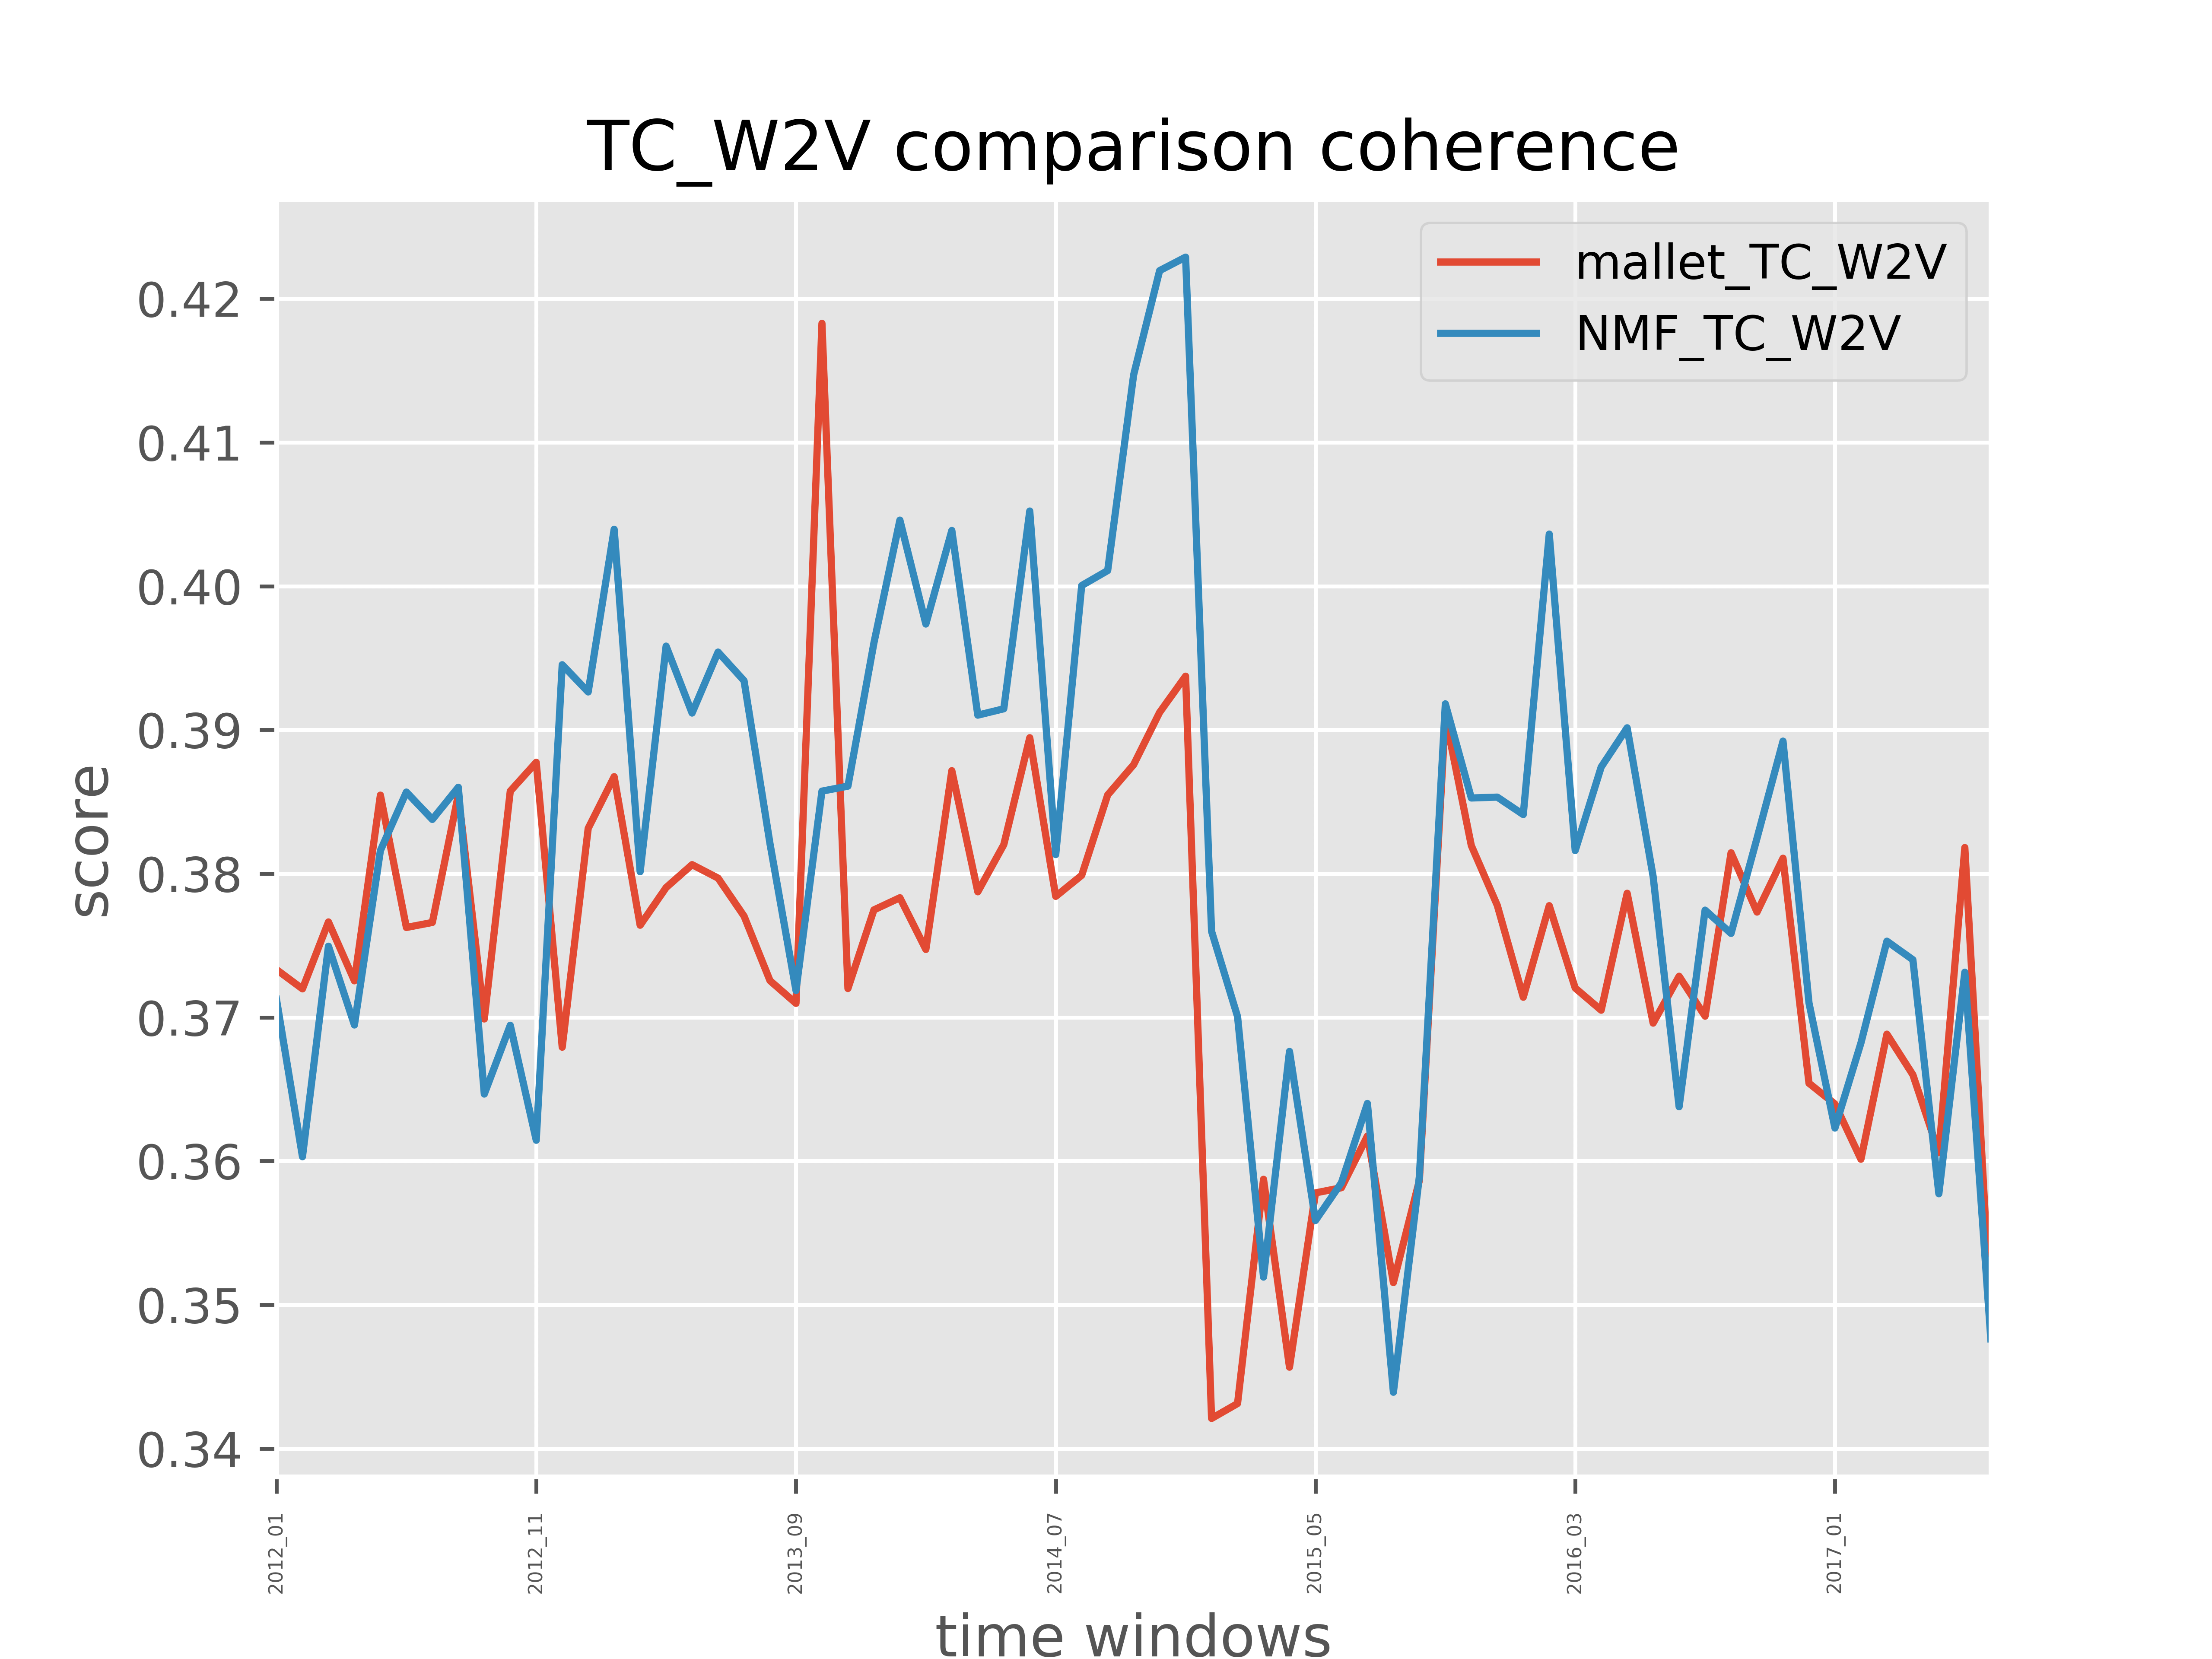
\includegraphics[width=\textwidth]{img/TC_W2V_comparison_all_coherence_plot.png}
  \end{minipage}
  \caption{Time window TC-W2V score comparison - LDA, LSA, LDA Mallet and NMF}
  \label{fig:window_TC_W2V_coherence_all}
\end{figure}

% Top K
\begin{figure}[!ht]
  \centering
  \begin{minipage}[b]{0.45\textwidth}
    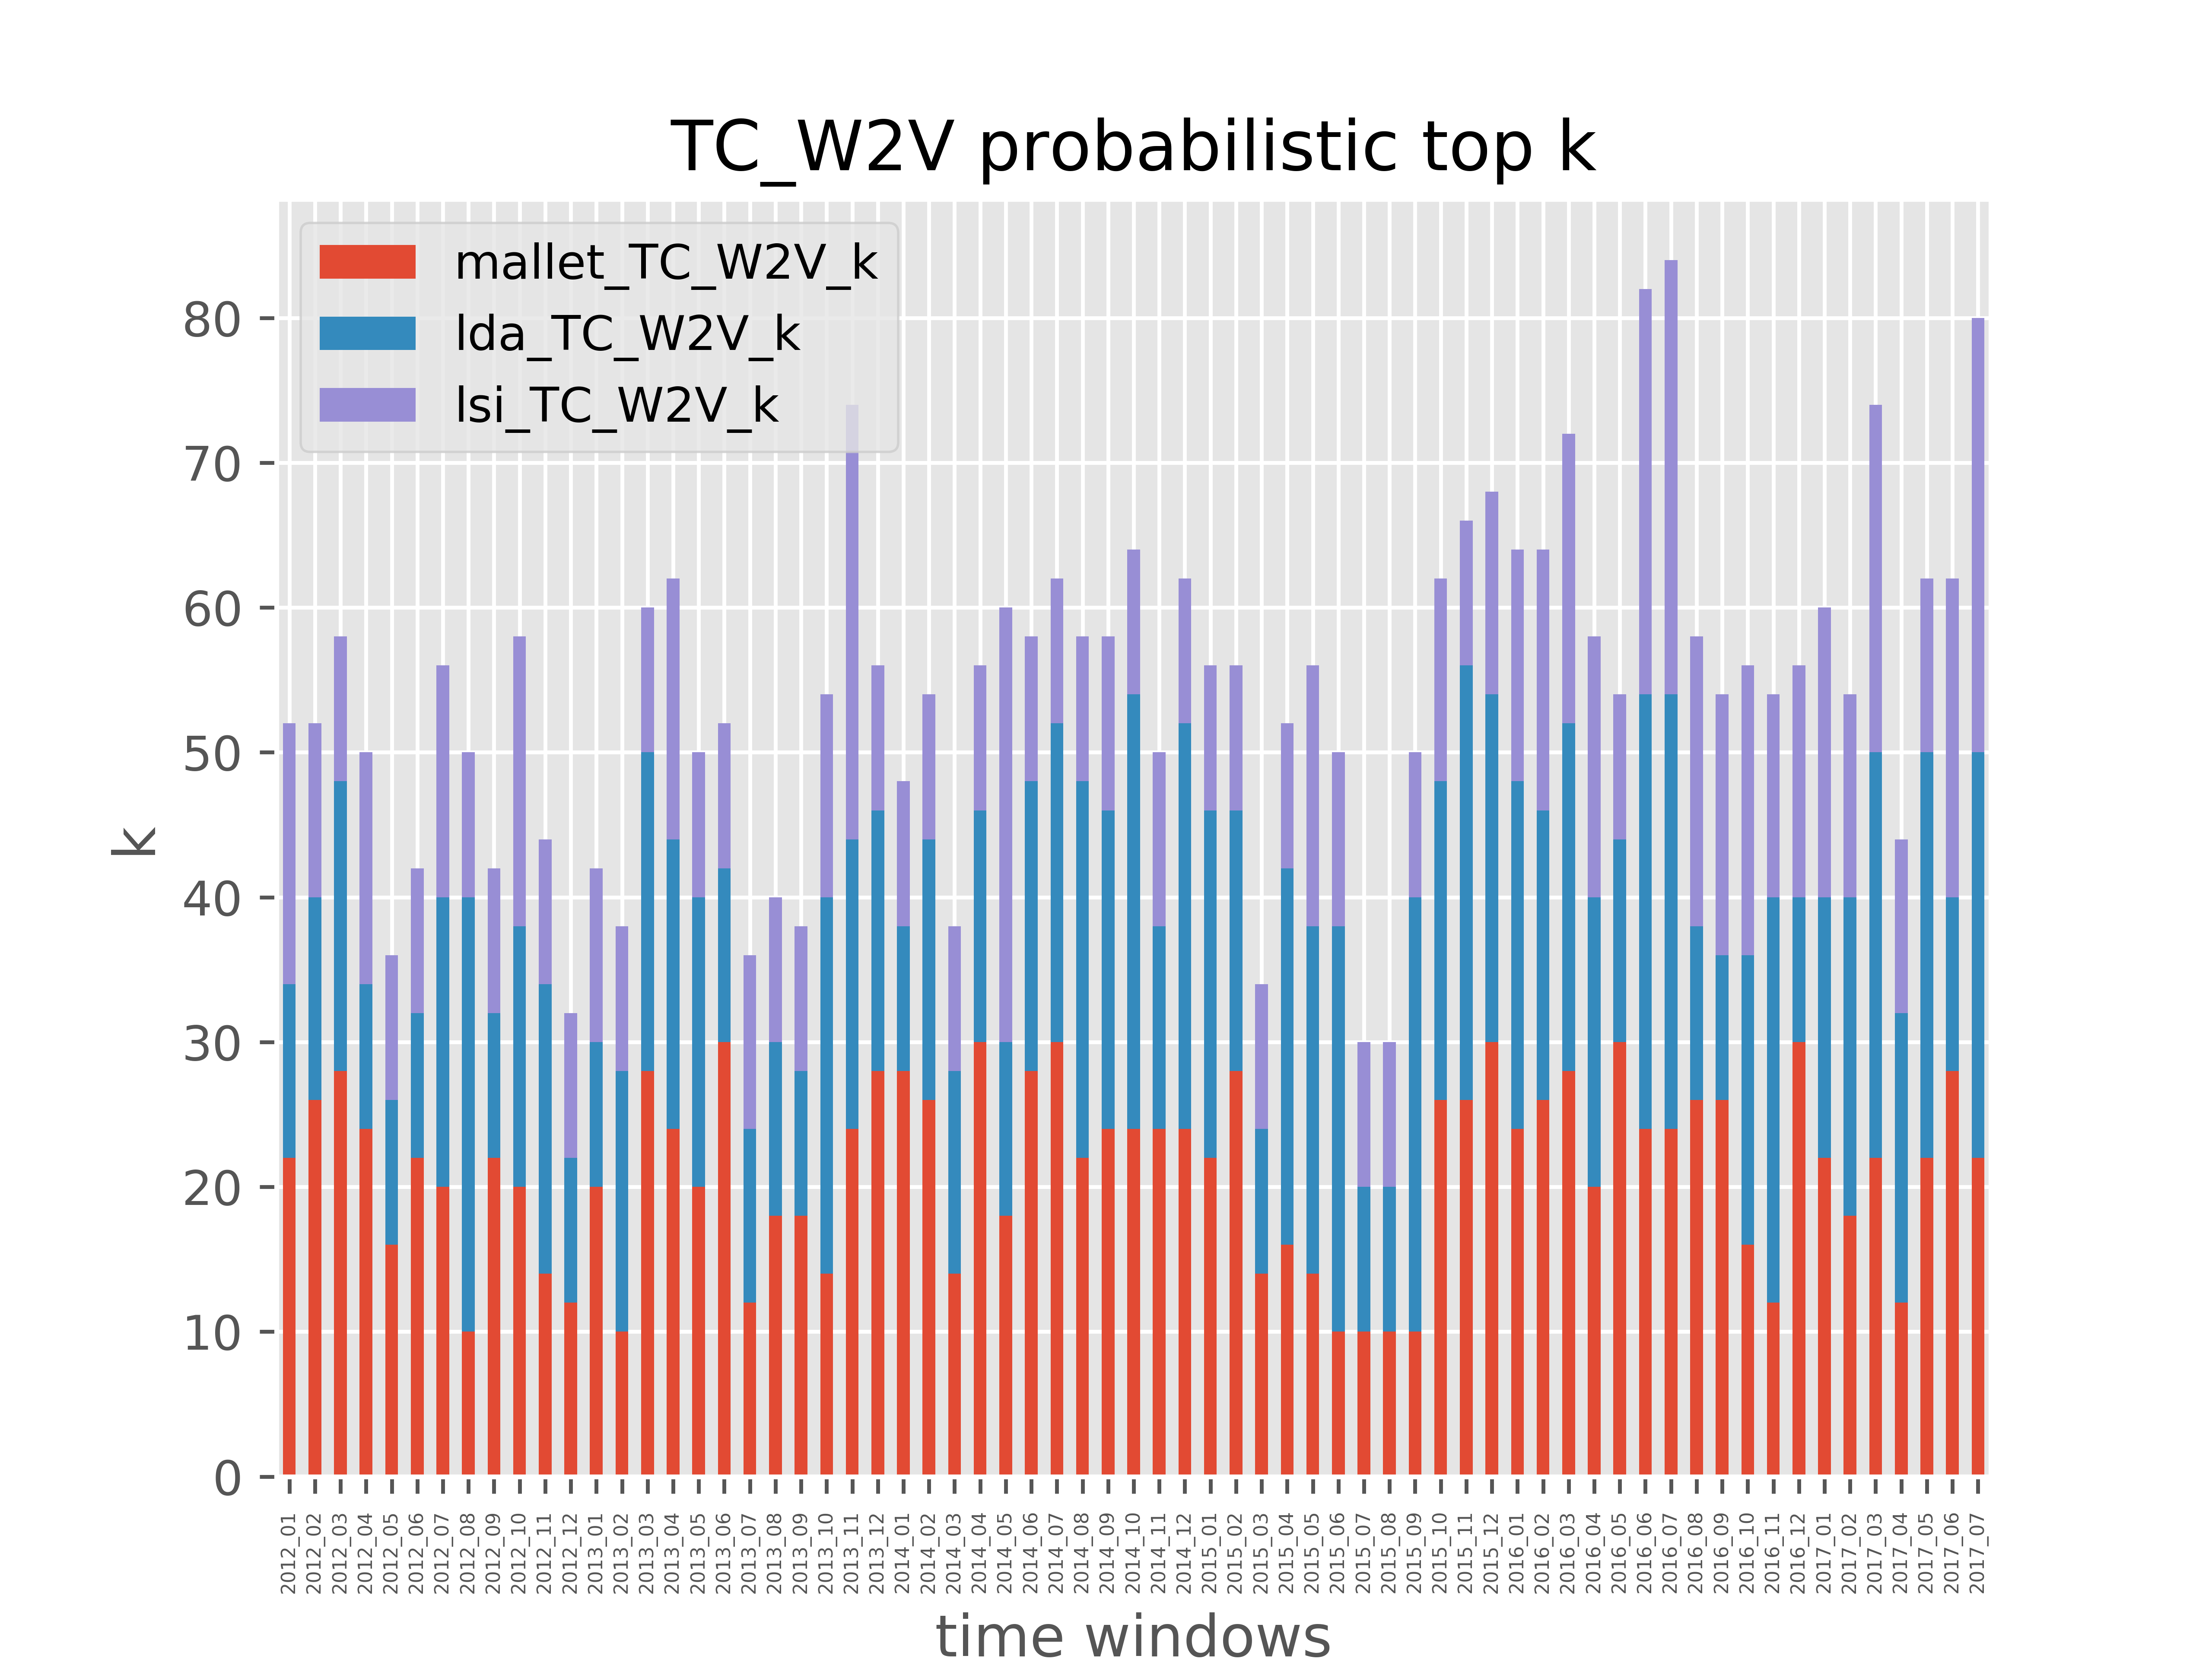
\includegraphics[width=\textwidth]{img/TC_W2V_probabilistic_top_k_all_topK_plot.png}
  \end{minipage}
  \hfill
  \begin{minipage}[b]{0.45\textwidth}
    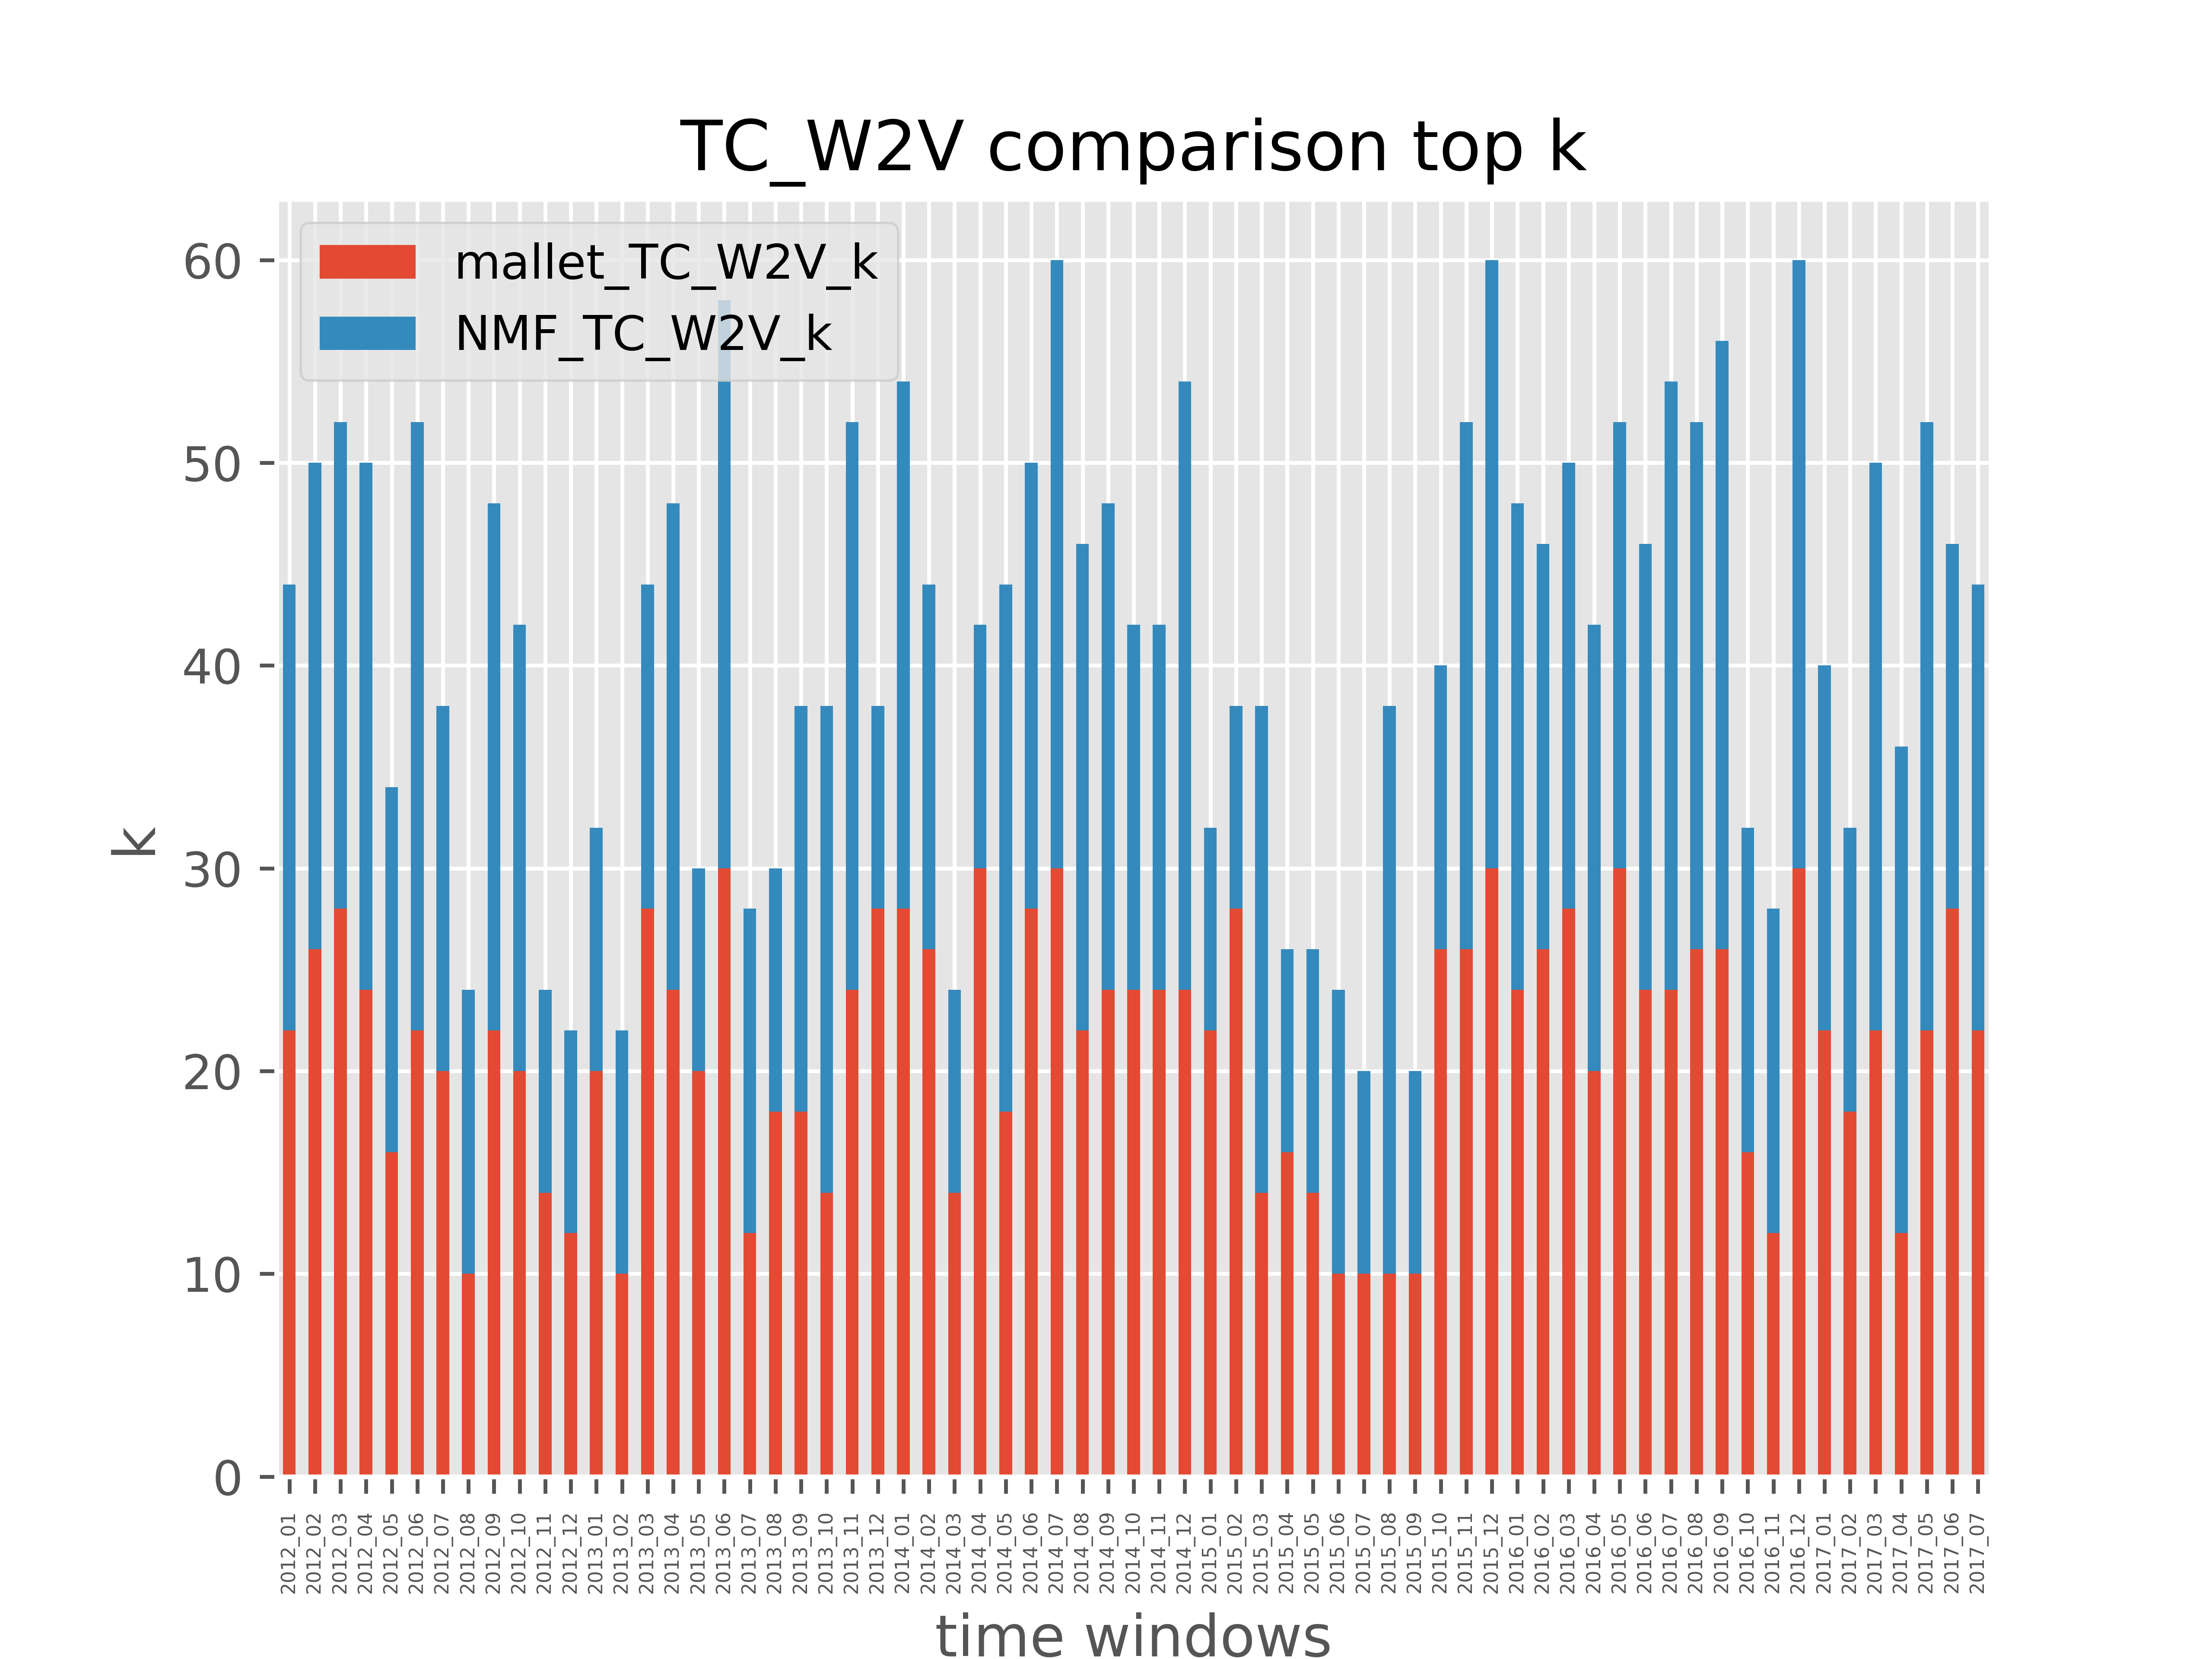
\includegraphics[width=\textwidth]{img/TC_W2V_comparison_top_k_all_topK_plot.png}
  \end{minipage}
  \caption{Time window TC-W2V top k - LDA, LSA, Mallet, NMF}
  \label{fig:window_TC_W2V_k_all}
\end{figure}


Statistically significant differences of coherence scores are determined using the two-tailed paired Student’s t-test computed  at  a  95\%  confidence  level. The performance of the LDA Mallet topic model coherence score is taken as strong baseline for this analysis. We analyze the improvements based on two difference coherence scores, TC-W2V and Unify coherence measure. In both cases, we observed statistically significant improvement coherence score. Figure \ref{fig:window_TC_W2V_coherence_all} and \ref{fig:window_Unify_coherence_all} shows the performance of the topic models across the window bins.

\begin{figure}[!ht]
  \centering
  \begin{minipage}[b]{0.45\textwidth}
    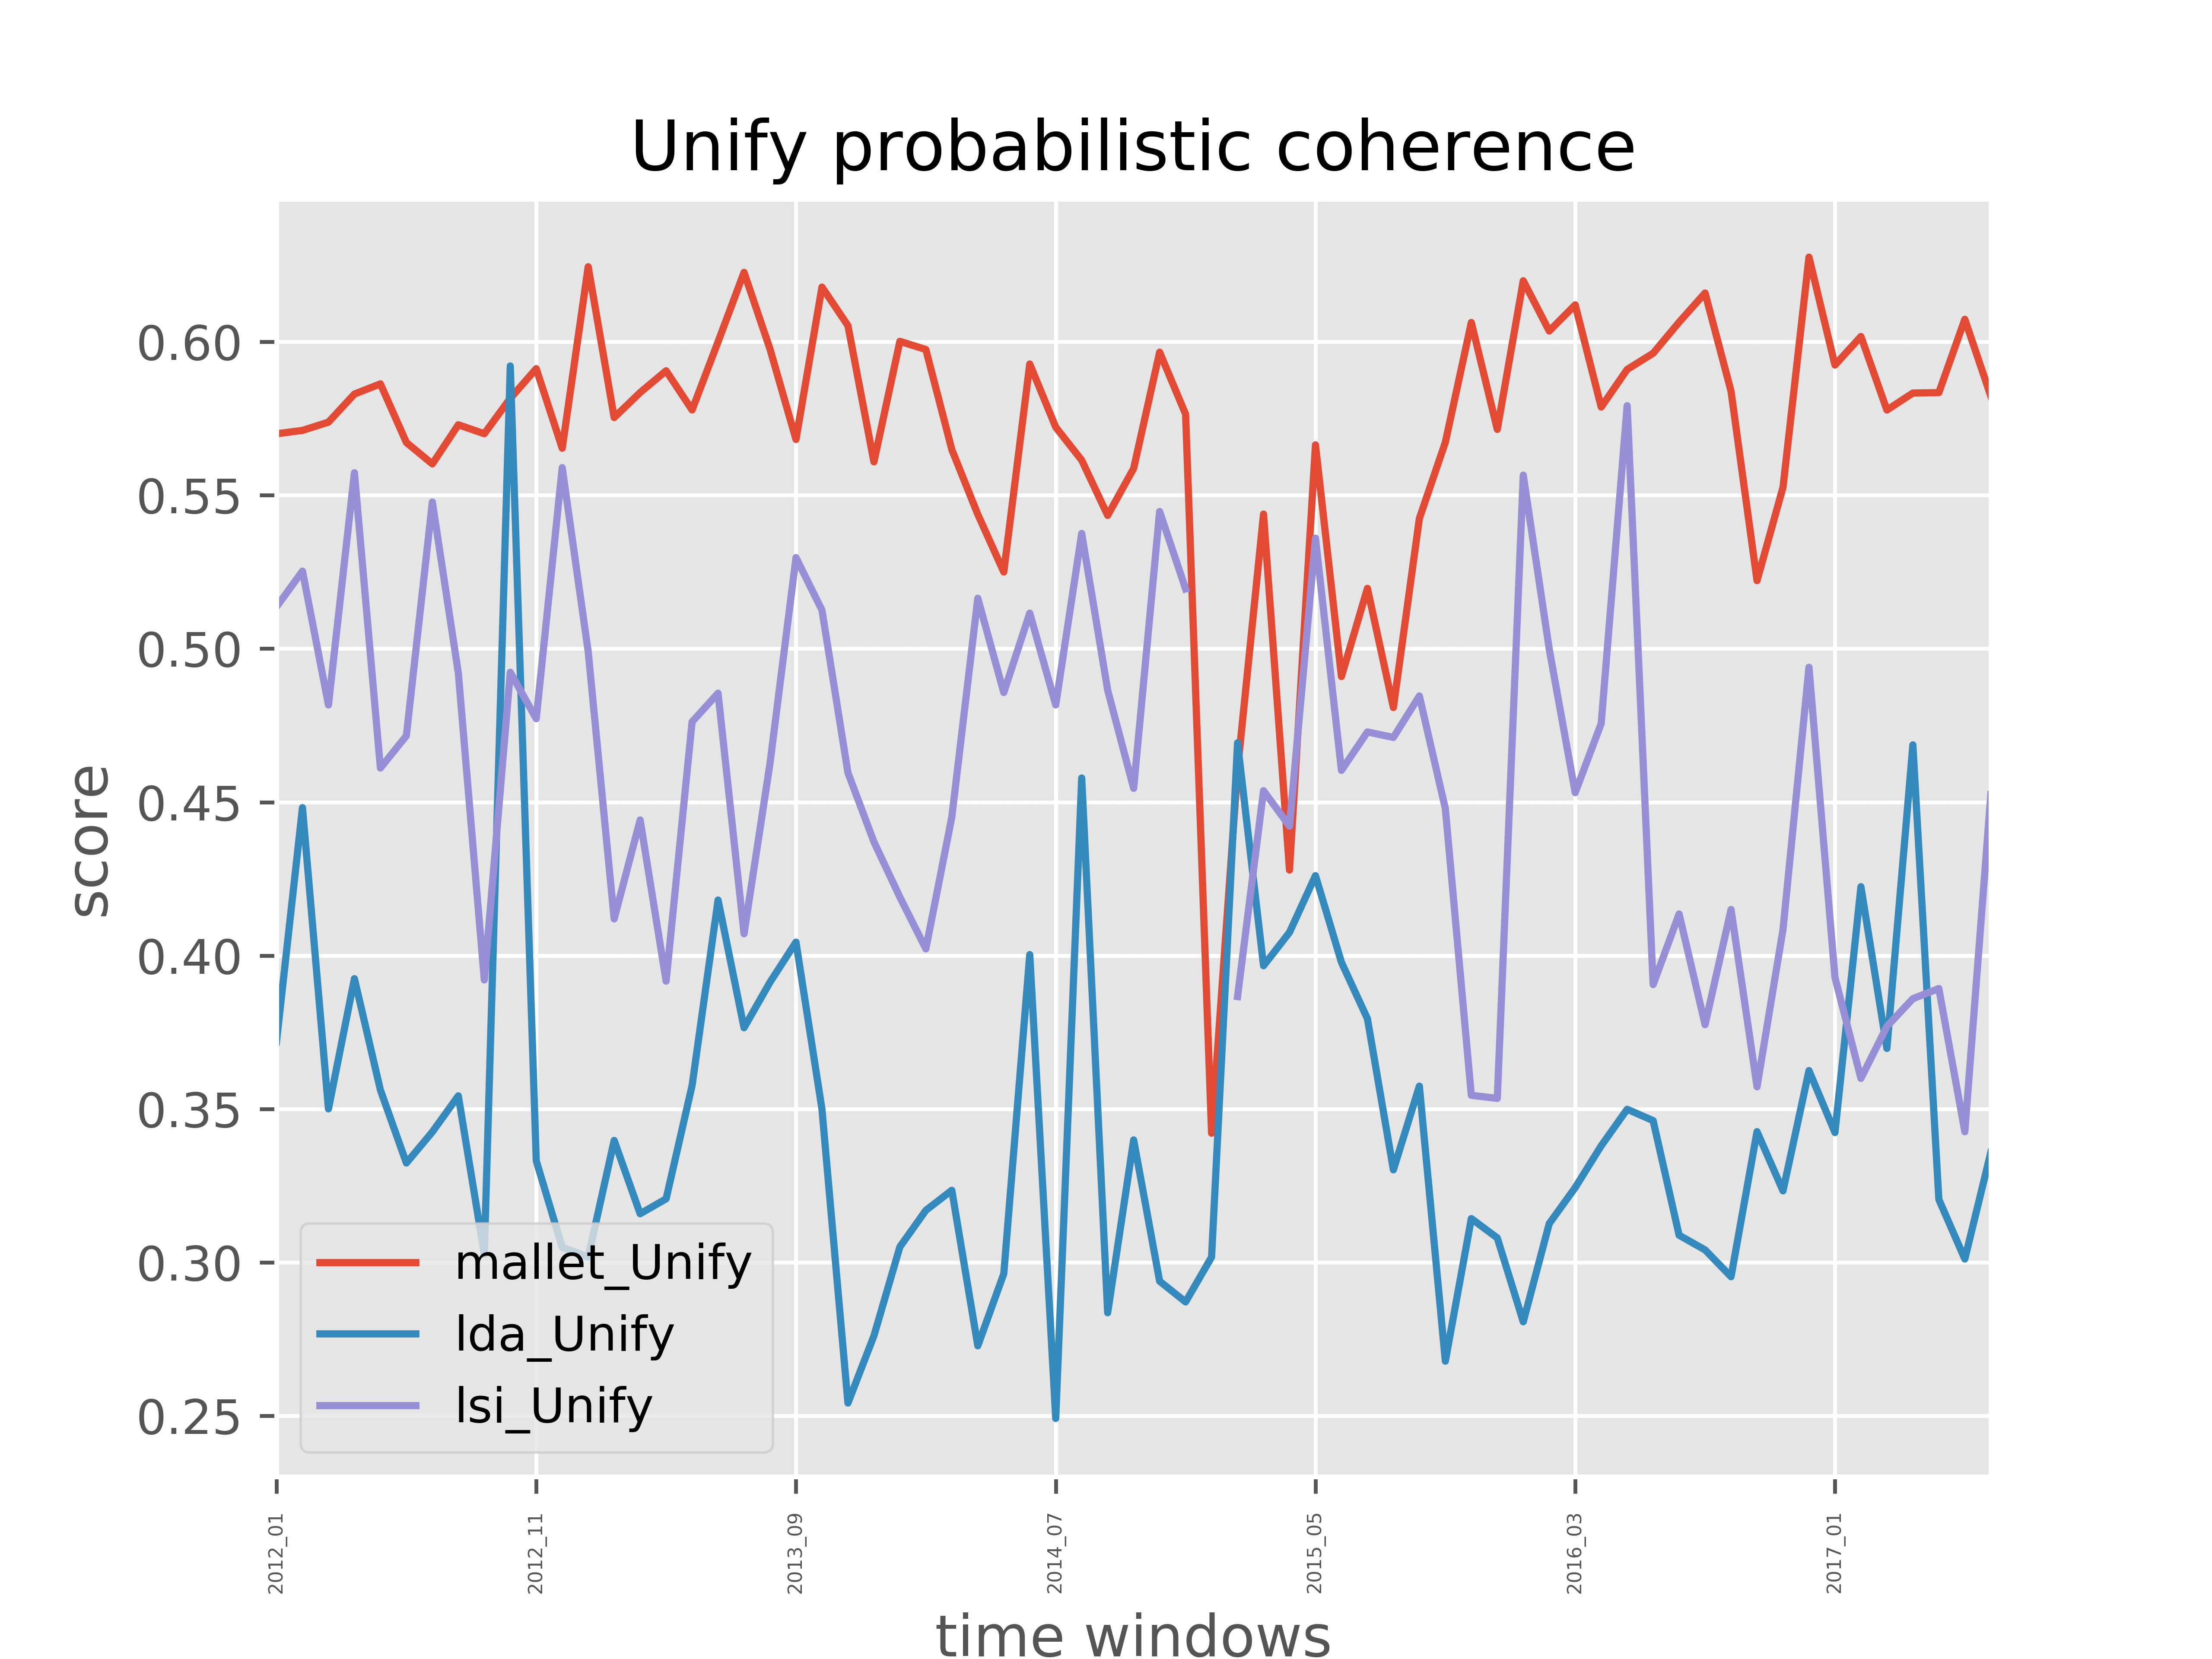
\includegraphics[width=\textwidth]{img/Unify_probabilistic_all_coherence_plot.png}
  \end{minipage}
  \hfill
  \begin{minipage}[b]{0.45\textwidth}
    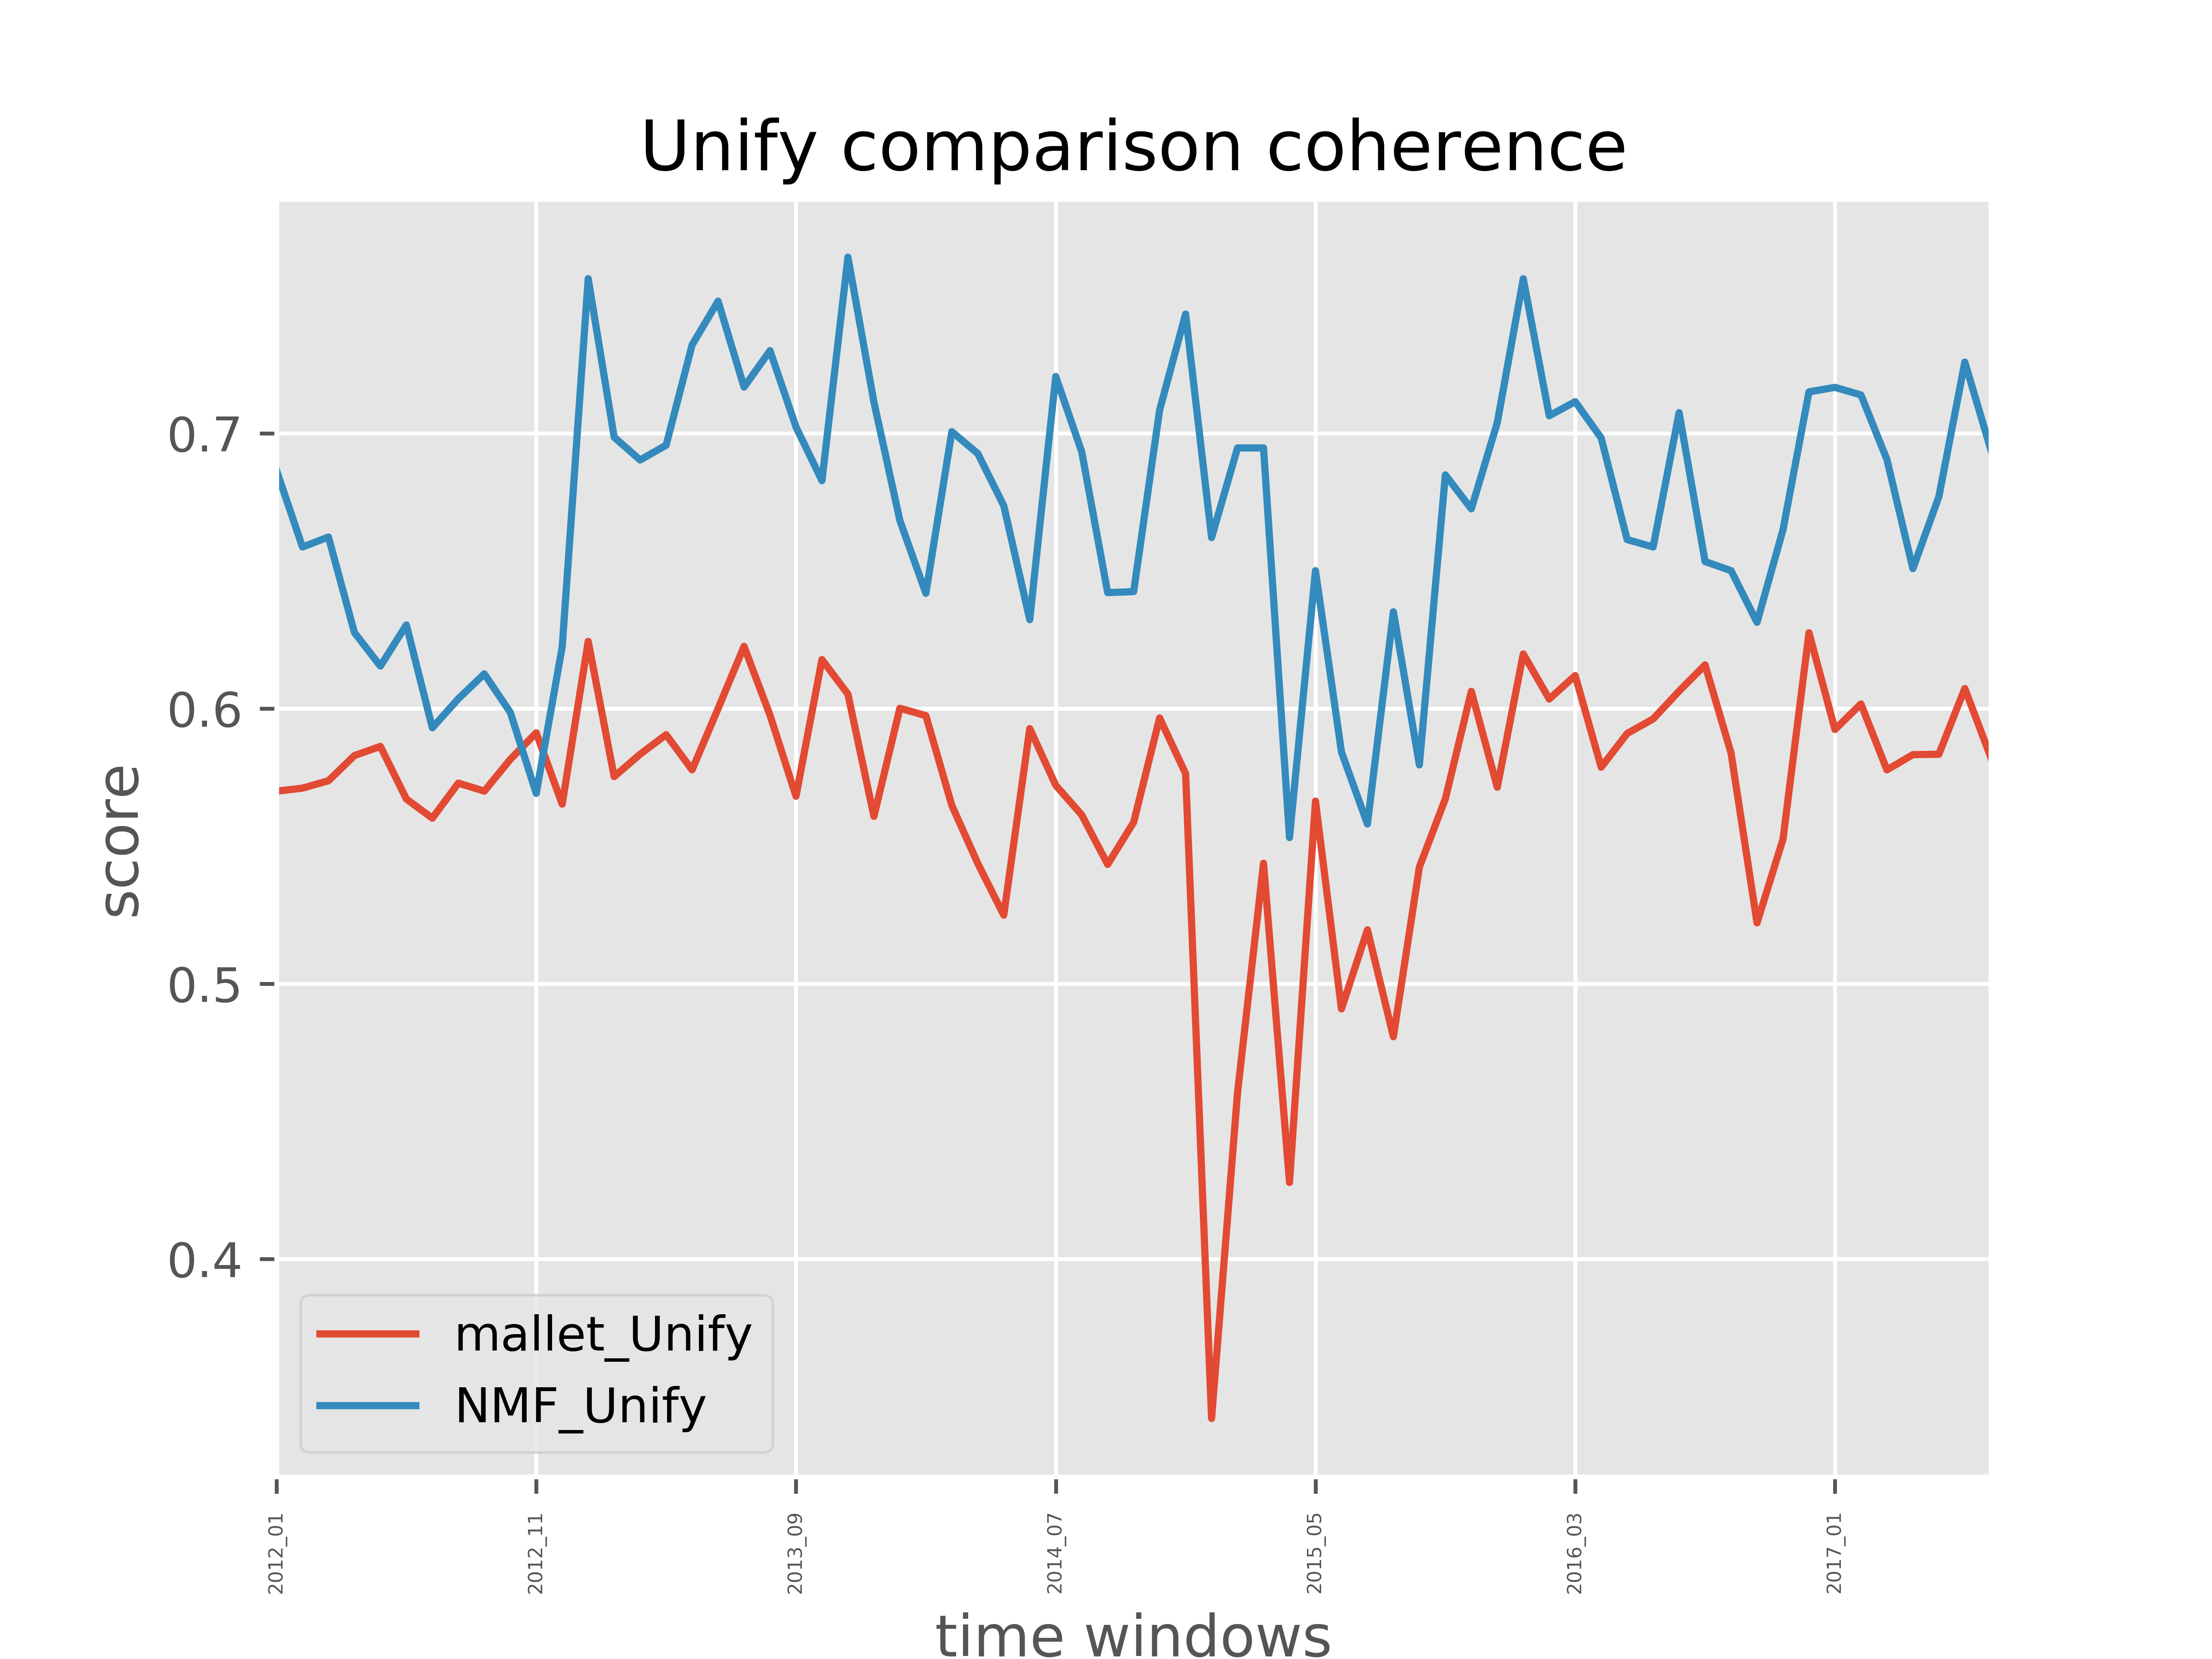
\includegraphics[width=\textwidth]{img/Unify_comparison_all_coherence_plot.png}
  \end{minipage}
  \caption{Time window Unify coherence - LDA, LSA, Mallet, and NMF}
  \label{fig:window_Unify_coherence_all}
\end{figure}

% Top K
\begin{figure}[!ht]
  \centering
  \begin{minipage}[b]{0.45\textwidth}
    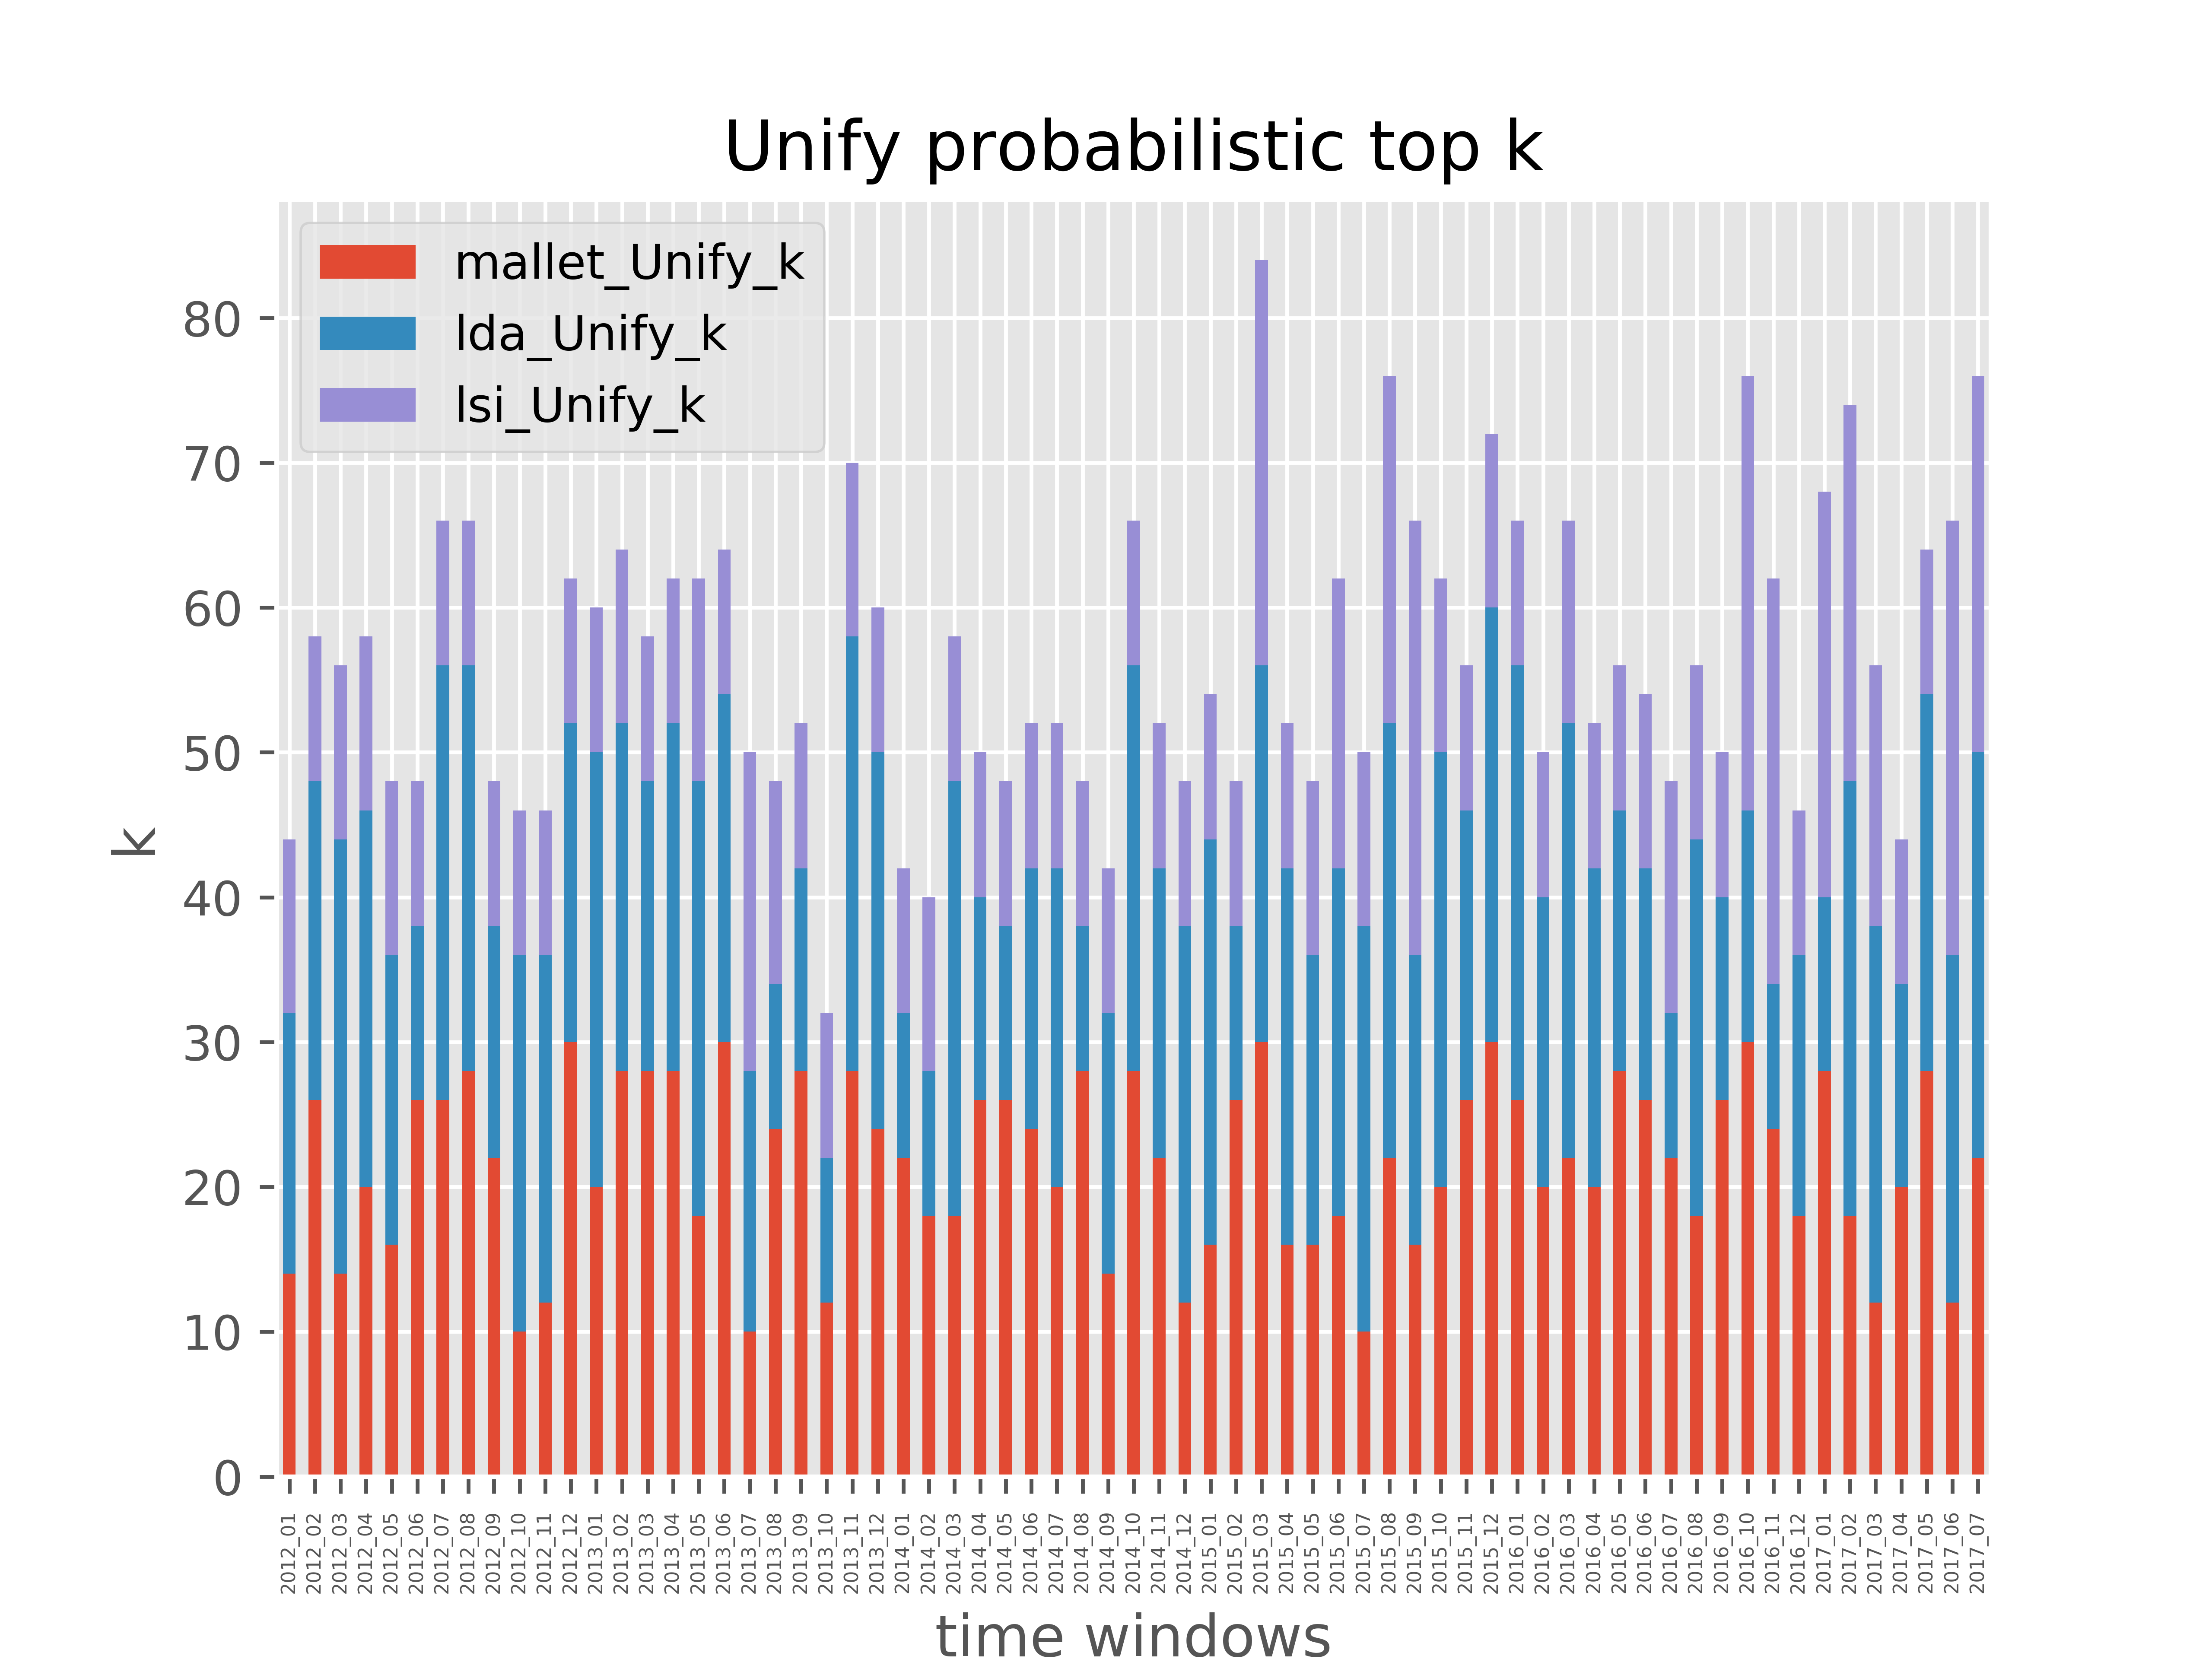
\includegraphics[width=\textwidth]{img/Unify_probabilistic_top_k_all_topK_plot.png}
  \end{minipage}
  \hfill
  \begin{minipage}[b]{0.45\textwidth}
    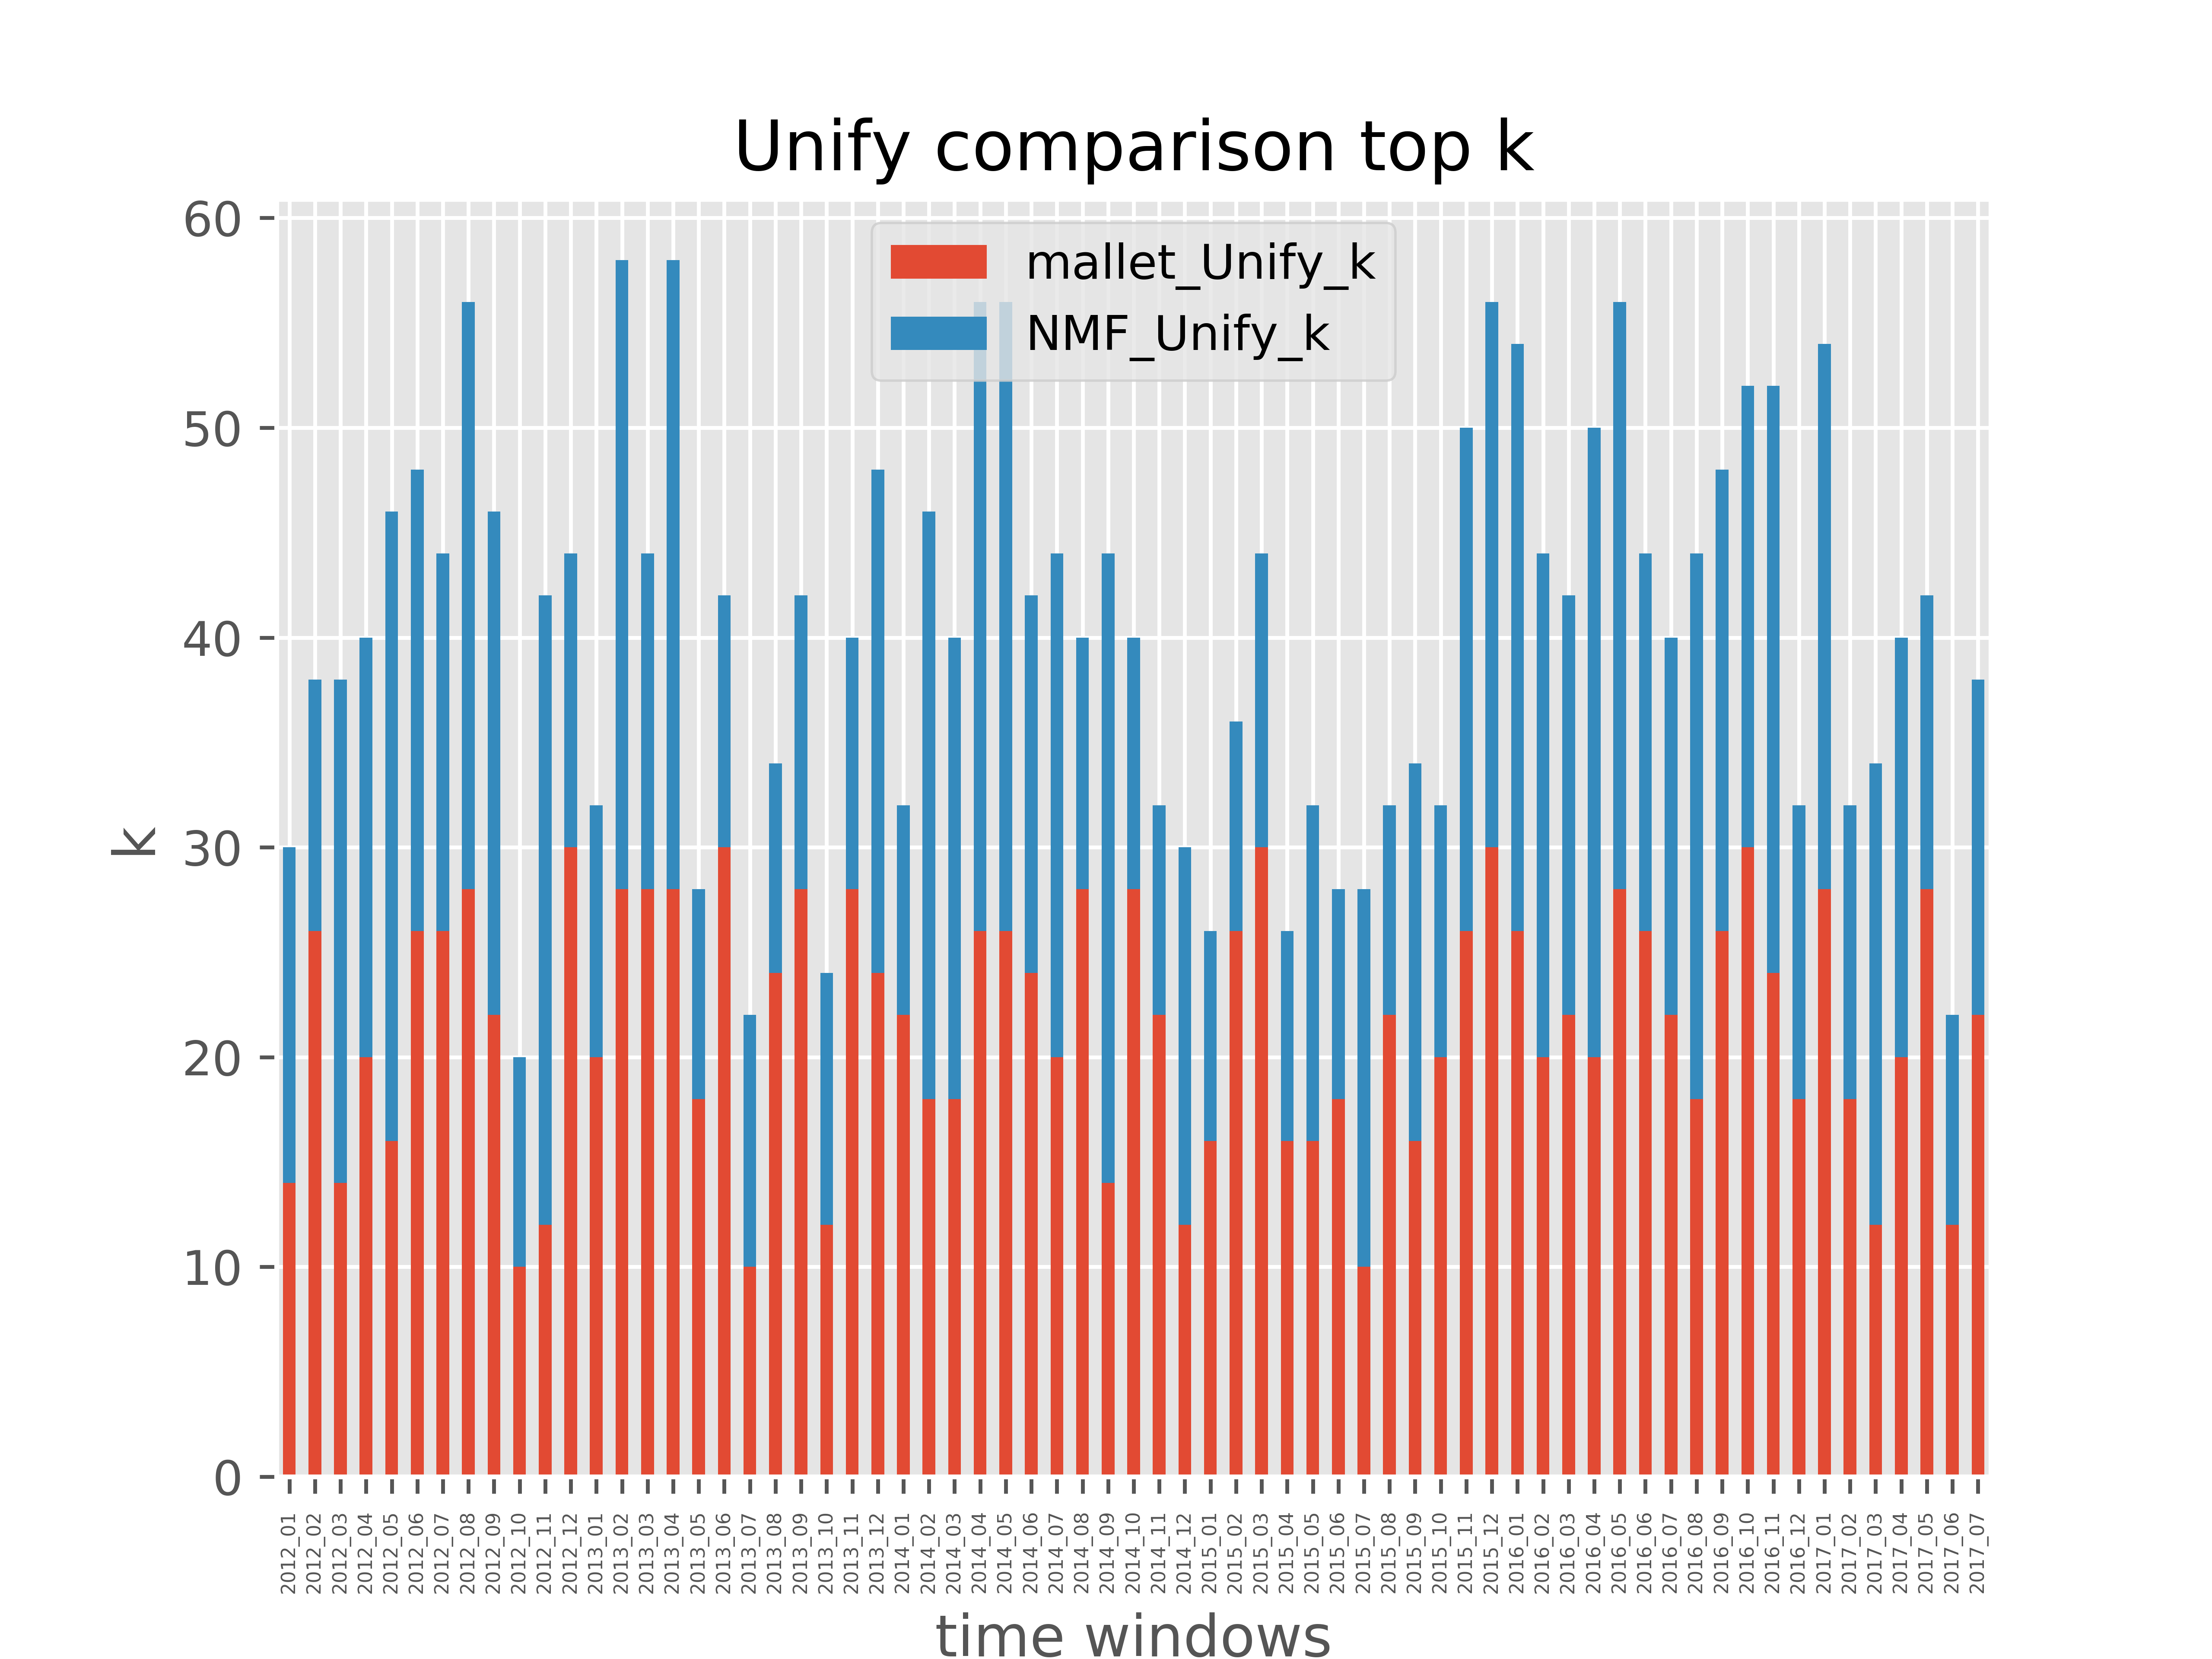
\includegraphics[width=\textwidth]{img/Unify_comparison_top_k_all_topK_plot.png}
  \end{minipage}
  \caption{Time window Unify top k - LDA, LSA, Mallet, and NMF }
  \label{fig:window_Unify_k_all}
\end{figure}




We can see that the NMF topic modeling shows improvements in the topic modeling coherence scores. This result is in agreements with the results discovered in \cite{Greene2016}. Another important advantage of the NMF, compare to the probabilistic approaches, is the speed of finding topics. The matrix factorization tends to be faster than it's counterpart probabilistic based approaches.


It is also interesting to note that LDA online variation based on \cite{NIPS2010_3902}, which is available as core component of the Python Gensim library, did not perform well compare to all other methods. The LDA Mallet is best performing amount the probabilistic approach, with LSA having the edge over the out of the box LDA topic models. 


The performance of the topic models heavily depends on the number of topics provided. Therefore, the key parameter selection decision involved in topic modeling is the choice of the number of topics $k$. To address this, the topics models are evaluated based on the topic coherence measures described in section 4.2. Figure \ref{fig:window_TC_W2V_k_all} and \ref{fig:window_Unify_k_all} shows the best performing number of topics k in the window bins. The topic coherence score is computed to find the best performing number of topics. The topic coherence results from unified coherence framework and TC-W2V is also used to validate the how the two score measurements agree on identifying the highest topic model. 

\subsection{Dynamic Topic learning}
Table \ref{table:dynamictopk} shows the top coherence score base on the unify metrics. Best number of topics are found in the center of the $k \in \{10, 100\}$ range, with 42 being the best performing number of topics. We also noticed that low and high number of topics don't perform well in the coherence measurements. 

\begin{table}[H]
\centering
\caption{Dynamic model top k performance}
\label{table:dynamictopk}
\begin{tabular}{|l|l|}
\hline
k  & Unify score \\ \hline
42 & 0.608       \\ \hline
44 & 0.606       \\ \hline
55 & 0.602       \\ \hline
\end{tabular}
\end{table}

We use the dynamic topic modeling technique introduced in \cite{Greene2016} and described in section 4.4. After processing the corpus into time windows and applying the pre-processing steps (described in section 5.2), the two layers of NMF are applied on the sliced corpus. The result of the two-layer dynamic topic modeling is first set of time window topic models $M \in \{M_1, ..., M_T\}$, and set of dynamic topics with association to the time windows. 
Determining on the number of topics is the most important part of any topic modeling. In these set of experiments, we set $k \in \{10, 100\}$ with the increments of 2. This range is used to generate topic models for each time period as well as generating the dynamic model. We use the unify topic coherence measure to decide on the best performing topic number for each period of time (Figure \ref{fig:topk_coherence_tc}).

% GRAPHS GO HEREh
\begin{figure}[H]
\centering
\caption{Dynamic unify top coherence}
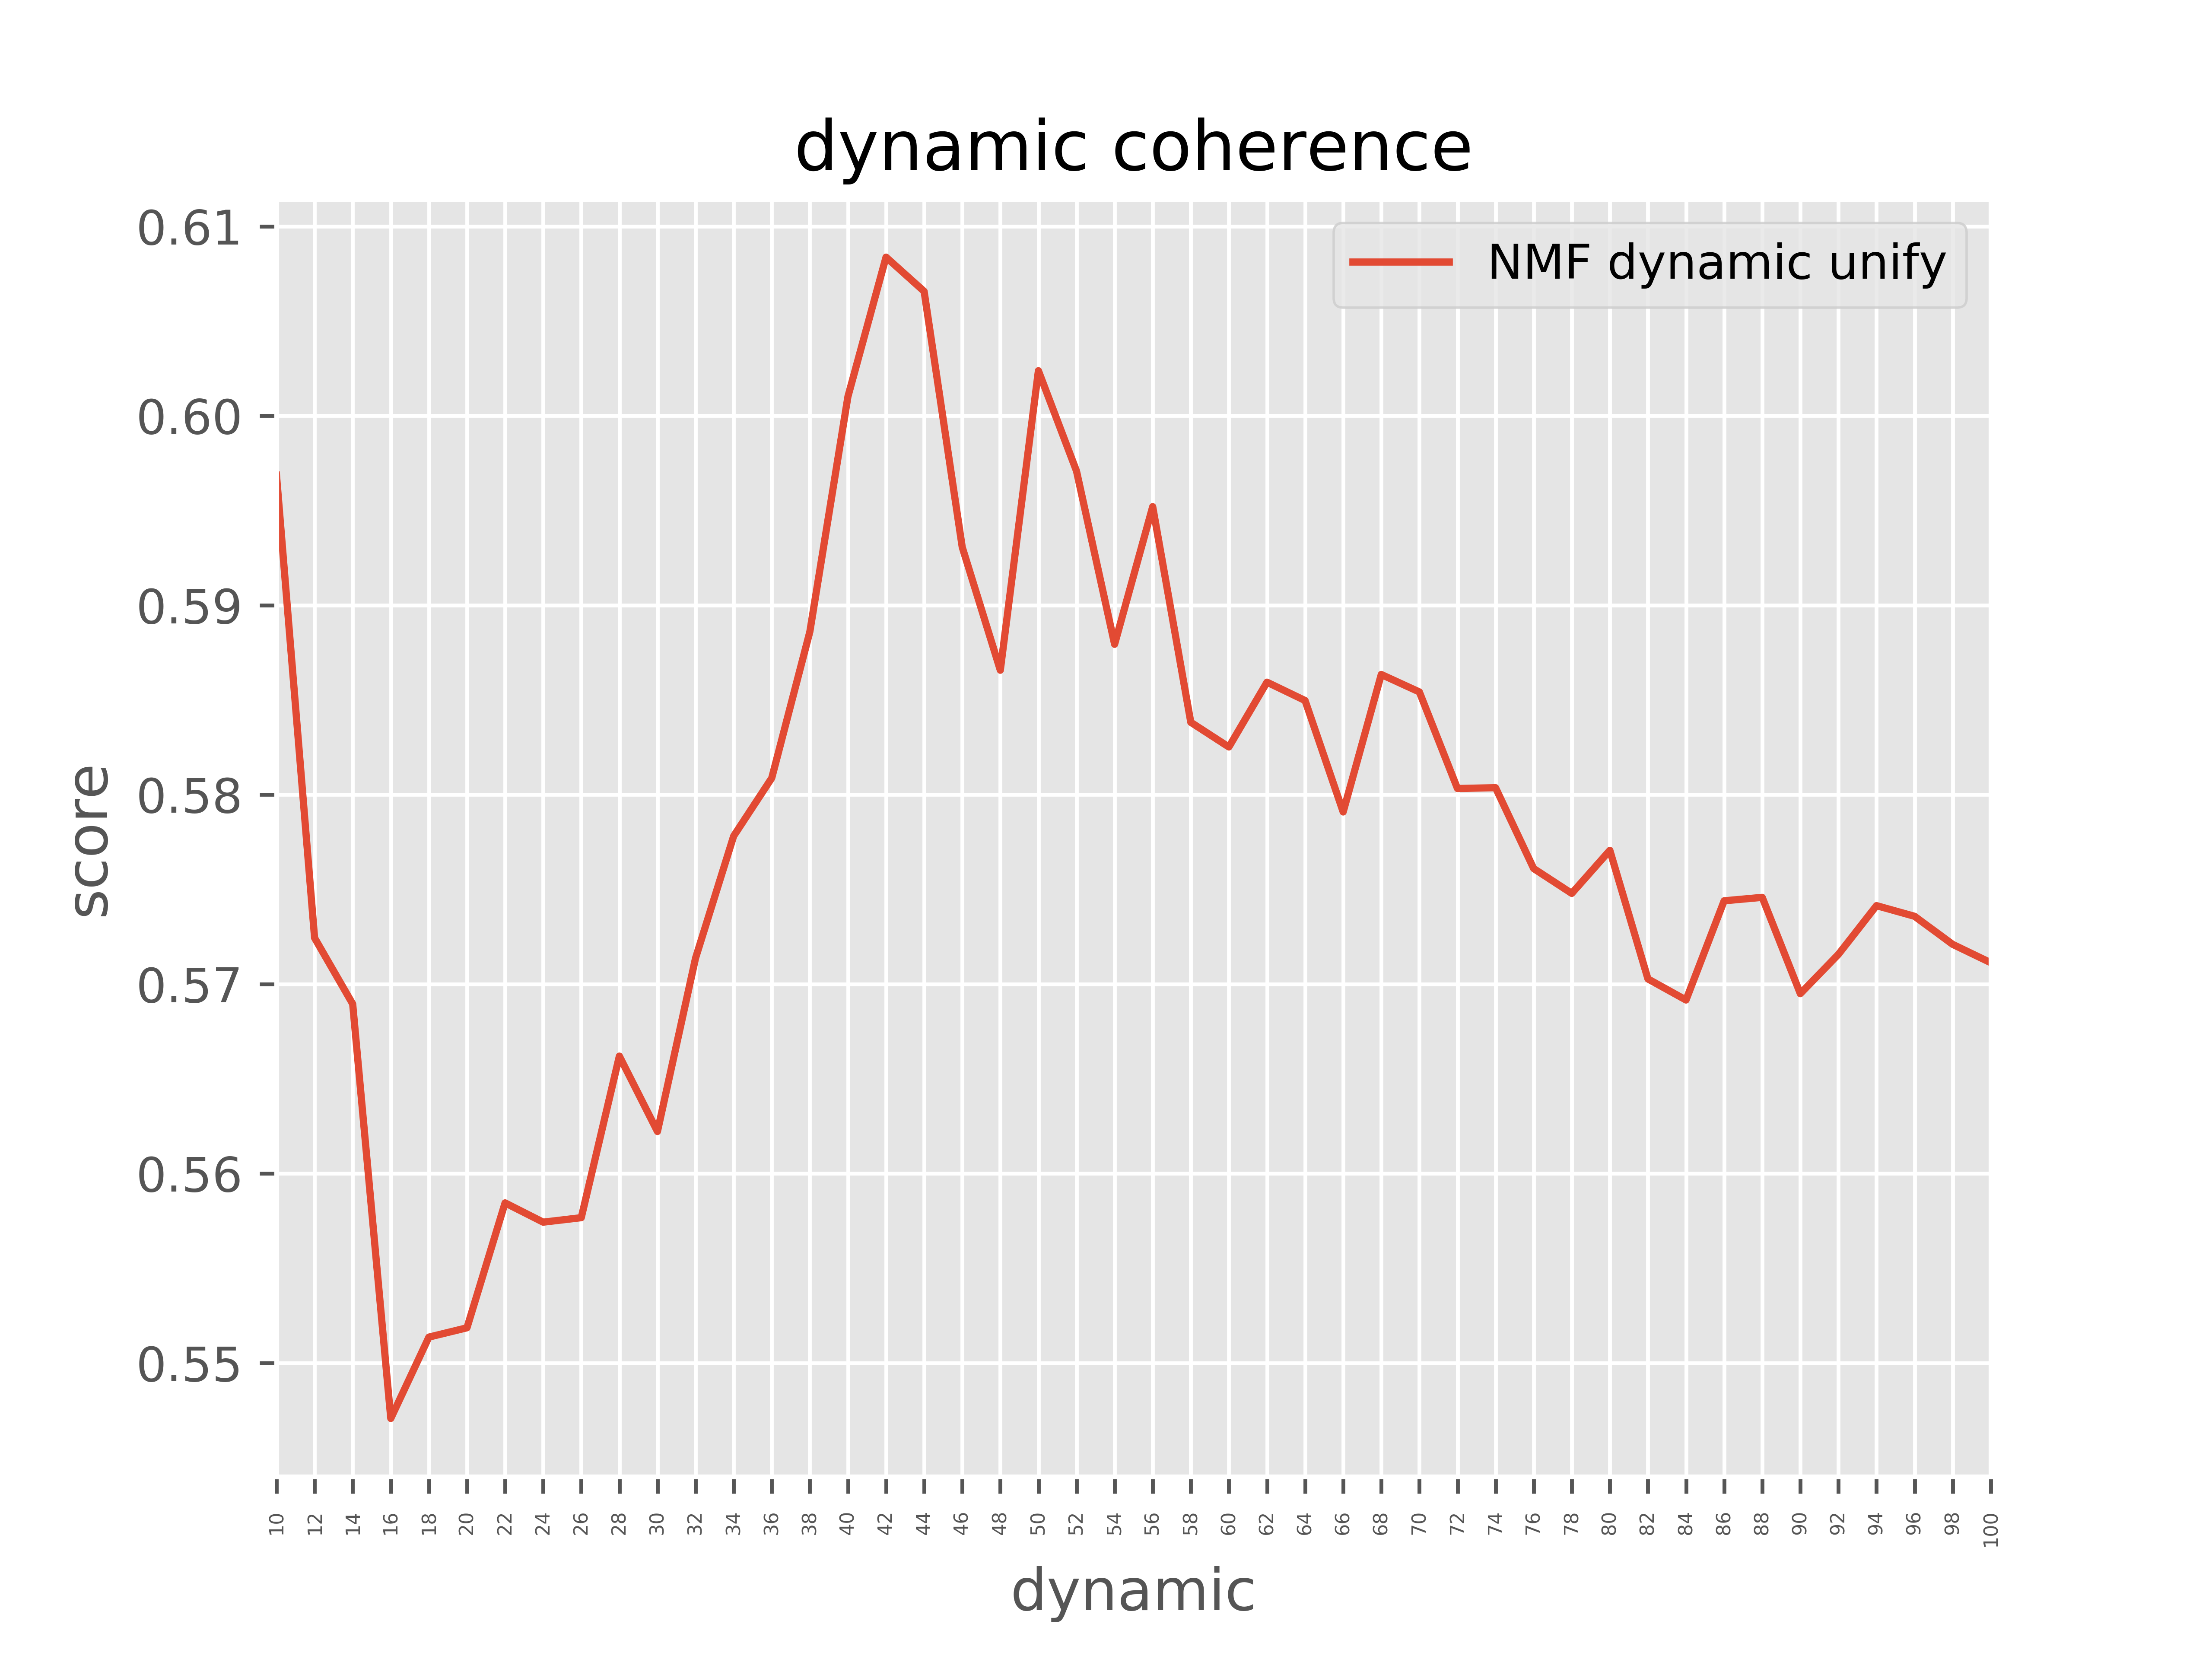
\includegraphics[scale=.7]{img/dynamic_coherence_plot.png}
\label{fig:topk_coherence_tc}
\end{figure}




We can also manually inspect the quality of the dynamic topics found in out news article corpus. Since the corpus was curated to focus on the Middle East, we can expect that the topics found center around the issues in the region. Exploring subset of the topic $k = 42$ (Table \ref{table:dynamictopicWords}) shows that the topics refer to set of ongoing events throughout the whole entire period of 2012-2017. 


\begin{table}[H]
{ \singlespacing
\small
\centering

\begin{tabularx}{\textwidth}{|l|X|}

 \hline
 Topic & Top 10 words   \\
 \hline\hline
 Syrian crisis &  refugee, child, million, Jordan, UNHCR, Syrian\_refugee, humanitarian, people, flee, aid\\
 \hline
 Syrian crisis &  chemical, weapons, Syria, OPCW, Syrian, attack, gas, destroy, prohibition, stockpile \\
 \hline
 Iraq conflict &  Mosul, Iraq, forces, city, Islamic\_state, Fallujah, troop, militant, daesh, retake \\
 \hline
 Syrian crisis &  council, resolution, Syria, security, united\_nations, Annan, observer, violence, mission, secretary\_general \\
 \hline
 Iraq conflict & killed, Baghdad, wound, car, attack, bomb, people, suicide, police, security
 \\ [1ex] 
 \hline
 
\end{tabularx}
\caption{Dynamic topics} \label{table:dynamictopicWords}
}
\end{table} 

\section{Case Study}
In this section, we will use a case study to elaborate more on the topic discovery in a large news media corpus. We investigate the topics emerging from the corpus with some population displacement factors identified in section 3. For this case, we focus on the topics related to rise of violent conflict by the Islamic extremist group ISIS/Daesh in Syria and Iraq. The selected topic and its top words are presented in Table \ref{tab:topicWords}. 

We start by looking at the events in early months of 2014. The Battle of Fallujah was among the earlier stages of territory lost to the ISIS and other Sunni insurgents. The City of Fallujah,  and the nearby city of Ramadi, the capital of Al Anbar Governorate, fell into hands of ISIS forced in early January as the Iraqi army forces withdrew from both cities.  As a consequence, most police forces abandoned their posts, leaving behind weapons and ammunition that was seized by ISIS. Fall of these cities led to Anbar Campaign to recaptured the cities in two years. 

We also notice various armed groups and coalitions joined the war against the Islamic State of Iraq (ISIS) that started on 2 January 2014. Its aim was to expel ISIS from the western Aleppo countryside. We can trace this conflict in the later months of 2014.

The international red line also resulted in Syrian government give up its chemical weapon arsenal. Syria delivered the first load of chemical weapons to its port city Latakia in January 2014. The chemical weapons were then loaded on a Danish ship that sailed out into international waters. 

In February 2014, the Syrian government allowed about 1,400 people to be evacuated from the Old Homs City. Baghdad also experiences a new wave of car bombs ripped through commercial areas, which resulted in tens of civilian casualties. Meanwhile, the Anbar Campaign continues with more civilian casualties.
Heads of Arab states are holding their annual summit in March 2014 to address the tension over the crisis in Egypt and the conflict in Syria and Iraq.


\begin{table}[H]
{ \singlespacing
\small
\centering

\begin{tabularx}{\textwidth}{|l|X|}

 \hline
 Topic & Top 30 words   \\
 \hline\hline
 2014/01 &  fallujah, ramadi, militant, city, forces, iraqi, anbar, security, control, sunni, anbar\_province, clashes, government, al\_qaeda, fighting, tribesman, link, protest, fighters, al\_qaida, say, police, area, tribal, iraq, isil, army, maliki, baghdad, camp \\
 \hline
 2014/01 &  chemical, weapons, opcw, syria, port, ship, material, danish, latakia, vessel, destroy, destruction, syrian, arsenal, prohibition, mission, escort, transport, chinese, will, removal, say, deadline, un, norwegian, remove, uzumcu, frigate, operation, sea  \\
 \hline
 2014/01 &  isil, rebel, rebels, group, aleppo, fighters, fighting, al\_qaeda, syria, activist, syrian, islamic\_state, observatory, jihadist, isis, say, northern, killed, raqqa, idlib, town, syrian\_observatory, opposition, rival, front, infighting, islamist, province, human\_rights, link  \\
 \hline
 2014/02 &  homs, aid, city, civilian, evacuate, red\_crescent, besiege, un, say, old, evacuation, food, people, syrian, rebel, convoy, area, trap, day, humanitarian, fire, barazi, leave, held, united\_nations, deliver, man, hom, siege, child  \\
 \hline
 2014/02 &  baghdad, iraq, killed, wound, car, police, militant, iraqi, bomb, people, say, least, attacks, sunni, violence, security, fallujah, city, ramadi, capital, source, killing, forces, anbar, near, official, gunman, area, bombs, blast  \\
 \hline
 2014/02 &  aleppo, rebel, group, isil, al\_qaeda, syrian, syria, say, barrel, fighters, killed, fighting, islamic\_state, observatory, assad, forces, isis, jihadist, al\_qaida, activist, opposition, held, regime, city, islamist, town, front, human\_rights  \\
 \hline
 2014/03 &  syrian, lebanon, rebels, syria, town, hezbollah, border, lebanese, say, rebel, assad, fighters, nun, yabroud, army, group, fighting, arsal, damascus, forces, area, president\_bashar, government, village, near, tripoli, al\_assad, regime, killed, yabrud  \\
 \hline
 2014/03 &  nina, ramadi, source, iraqi, fallujah, baghdad, police, wound, agency, end, security, al, national, civilian, news, city, killed, anbar, area, tikrit, kirkuk, tell, bomb, armed, elements, two, isis, army, gunman, reporter
  \\
 \hline
 2014/03 & arab, summit, kuwait, qatar, league, egypt, saudi\_arabia, state, gulf, al, opposition, muslim\_brotherhood, political, seat, support, call, country, syria, bahrain, leader, syrian, jarba, iraq, coalition, doha, minister, solution, egyptian, saudi, say
 \\ [1ex] 
 \hline
 
\end{tabularx}
\caption{Time window topics} \label{tab:topicWords}
}
\end{table} 